\documentclass[12pt]{article}
\usepackage[T1]{fontenc}
\usepackage[T1]{polski}
\usepackage[utf8]{inputenc}
\usepackage{color}
\usepackage{graphicx}
\usepackage{blindtext}
\usepackage{scrextend}
\newcommand{\BibTeX}{{\sc Bib}\TeX} 
\usepackage{graphicx}
\usepackage{amsfonts}

\setlength{\textheight}{21cm}

\title{{\bf Zadanie nr 3 - Splot, filtracja i korelacja sygnałów}\linebreak
Cyfrowe Przetwarzanie Sygnałów}
\author{Aneta Wiśniewska, 204029 \and Hanna Paluszkiewicz, 203962}
\date{14.05.2018}

\begin{document}
\clearpage\maketitle
\thispagestyle{empty}
\newpage
\setcounter{page}{1}
\section{Cel zadania}

Celem ćwiczenia jest zapoznanie się w praktyce z procesami splotu, filtracji i korelacji sygnałów.

\section{Wstęp teoretyczny}

\subsection{Teoria}


\addtokomafont{labelinglabel}{\sffamily}

\begin{labeling}{alligator}

%%%%%%%%%%%%%%%%%%%%%%%%%%%SPLOT%%%%%%%%%%%%%%%%%%%%%%%%%%%%%%%%%%%%%%%%%%%%%%%%

\item [Splot] to jedno z najważniejszych działań podczas filtracji sygnałów dyskretnych. Jest operacją przetwarzania dwóch sygnałów, w wyniku której otrzymujemy pojedyńczy sygnał dyskretny.  W ogólnym przypadku splot jest zdefiniowany wzorem:
\begin{figure}[h!]
 \centering
 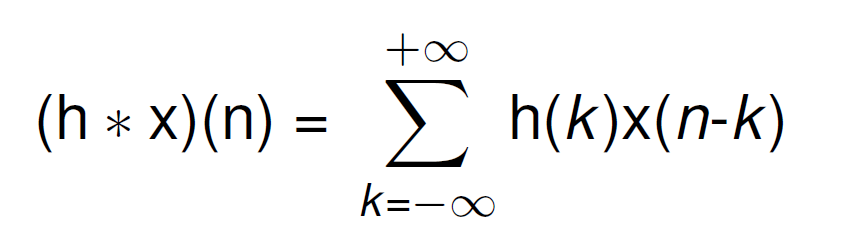
\includegraphics[width=6.3cm]{splotWO.PNG}
 \vspace{-0.3cm}
 \label{Widok_aplikacjis}
\end{figure}
W praktyce stosuje się sygnały o skończonych ilosciach próbek rozmieszczonych równomiernie w dowolnych miejscach osi czasu. Zwykle przyjmuje się konwencję indeksacyjną, gdzie oba sygnały zaczynają się  na osi czasu od próbki zero. Poza granicami przedziału oba sygnały są zerowe. 
\\Wzór dla tej konwencji przyjmuje postać: 
\begin{figure}[h!]
 \centering
 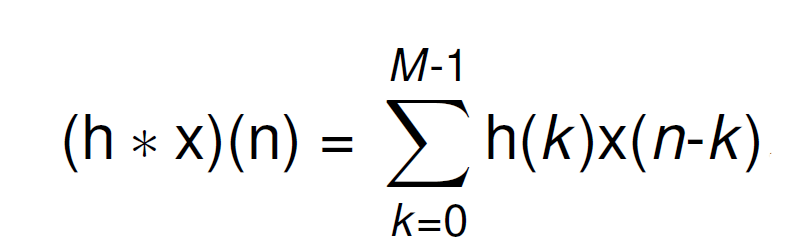
\includegraphics[width=6.3cm]{splotWS.PNG}
 \vspace{-0.3cm}
 \label{Splot_indeks}
\end{figure}

%%%%%%%%%%%%%%%%%%%%%%%%FILTRACJA%%%%%%%%%%%%%%%%%%%%%%%%%%%%%%%%%%%%%%%%%%%%%%%%

\item [Filtracja sygnałów]  - należy do podstawowych operacji CPS. W ramach filtracji widmo sygnału ulega modyfikacji. Zostały odfiltrowane składowe częci sygnału o częstotliwosciach należących do pasma zaporowego. Reszta widma leżąca w pamie przepustowym, nie uległa zmianie lub podlega niewielkiemu tłumieniu. 
\\Filtry ze względu na umiejscowienie pasma przepustowego i zaporowego dzielimy na:
\subitem Filtry dolnoprzepustowe - ich pasma przepustowe są okrelone przedziałem częstotliwosci od 0 do f0 (f0 - częstotliwosć odcięcia filtru) 
\subitem Filtry górnoprzepustowe - ich pasma przepustowe są okrelone przedziałem częstotliwosci od f0 do fp/2 (fp - częstotliwosć próbkowania sygnału) 
\subitem Filtry pasmowe - ich pasma przepustowe są okrelone przedziałem częstotliwosci od fd do fg (fd, fg > 0, fd < fg i fd, fg < fp/2) 

W zadaniu są stosowane filtry SOI - o skończonej odpowiedzi impulsowej. Zaletą tych filtrów jest łatwosć implementacji (w oparciu o splot) i projektowania postaci filtru. 
\\Przy obliczaniu próbki sygnału wyjsciowego (y(n)) jest brane pod uwagę M przeszłych próbek sygnału wejsciowego (x(n)). Wartosci y(n) obliczamy jako sumy ważone x(n) z uwzględnieniem współczynników filtru h(n). 
\\Opisuje to wzór:

\begin{figure}[h!]
 \centering
 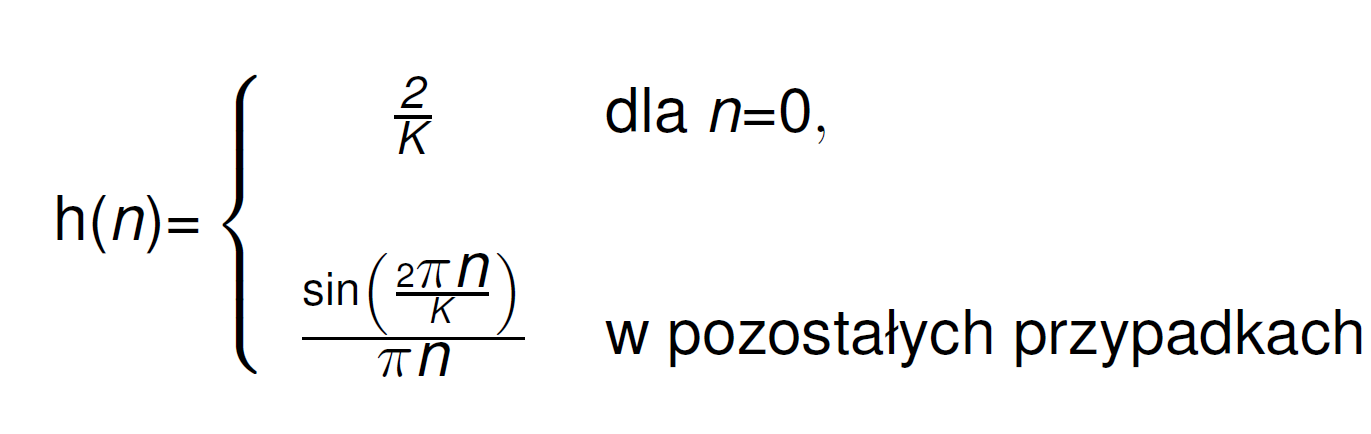
\includegraphics[width=9.3cm]{filtrS.PNG}
 \vspace{-0.3cm}
 \label{Splot_indeks}
\end{figure}

Gdzie:
\subitem M - rząd filtru
\subitem h(k) - odpowiedź impulsowa

Jeżeli ciąg próbek sygnału wejsciowego będzie ciągiem wartosci zerowych,  filtr SOI będzie generował na wyjsciu skończony ciąg niezerowych wartosci.

Powyższy wzór jest stosowany dla filtru dolnoprzepustowego. Na jego podstawie można obliczyć także działanie innych filtrów. W tym celu stosuje się wzory:
\subsubitem dla filtru srodkowoprzepustowego:
\begin{figure}[h!]
 \centering
 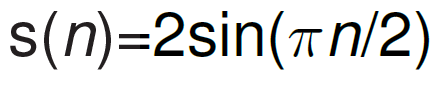
\includegraphics[width=3.3cm]{sr.PNG}
 \vspace{-0.3cm}
 \label{Splot_indeks}
\end{figure}

\subsubitem dla filtru górnoprzepustowego:
\begin{figure}[h!]
 \centering
 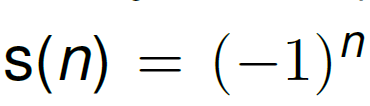
\includegraphics[width=3.3cm]{gor.PNG}
 \vspace{-0.3cm}
 \label{Splot_indeks}
\end{figure}


Do projektowania filtrów SOI została zastosowana metoda okna.


W praktyce często stosuje się okna:
\subitem Hamminga
\newpage
\begin{figure}[h!]
 \centering
 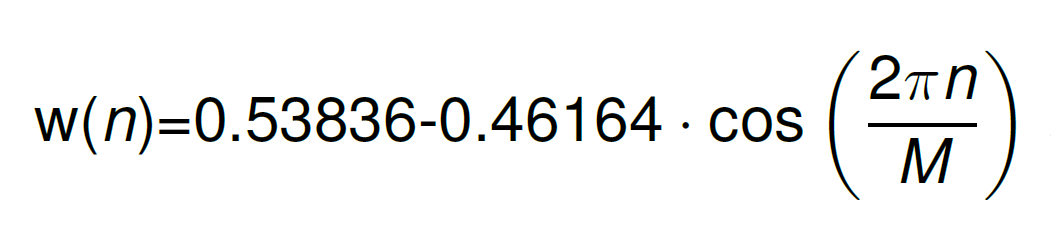
\includegraphics[width=6.3cm]{Hm.PNG}
 \vspace{-0.3cm}
 \label{gw}
\end{figure}

\subitem Hanninga

\begin{figure}[h!]
 \centering
 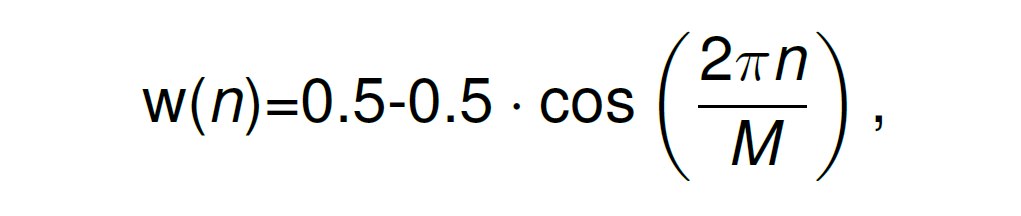
\includegraphics[width=6.3cm]{Hn.PNG}
 \vspace{-0.3cm}
 \label{gw}
\end{figure}

\subitem Blackmana

\begin{figure}[h!]
 \centering
 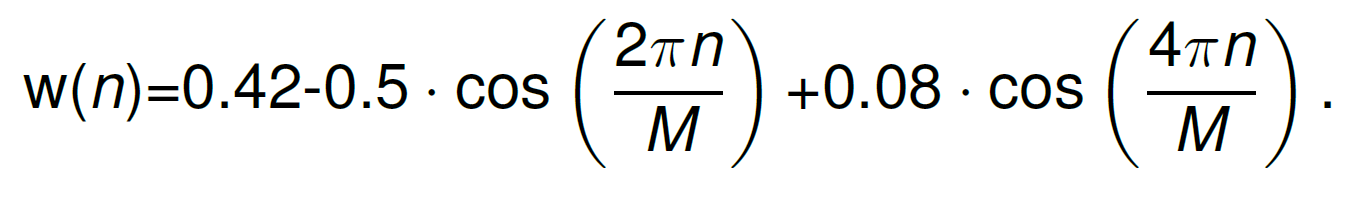
\includegraphics[width=7.3cm]{B.PNG}
 \vspace{-0.3cm}
 \label{gw}
\end{figure}

%%%%%%%%%%%%%%%%%%%%%%%%KORELACJA%%%%%%%%%%%%%%%%%%%%%%%%%%%%%%%%%%%%%%%%%%%%%%%%

\item [Korelacja] - jest ważną częscią przetwarzania sygnałów. Jest stosowana, gdy trzeba porównać sygnał z innym, zwłaszcza z przesuniętą na osi czasu swoją kopią.
Polega na przetwarzaniu dwóch sygnałów dyskretnych, w czego wyniku otrzymujemy pojedynczy sygnał dyskretny.
\\Korelacja w ogólnym przypadku jest opisywana wzorem:
\begin{figure}[h!]
 \centering
 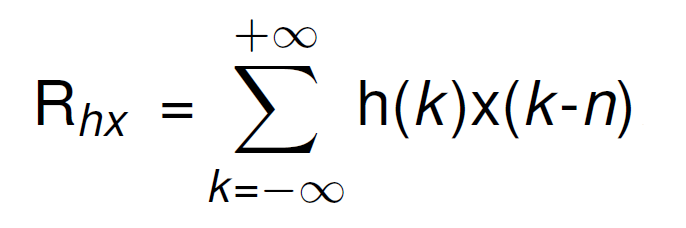
\includegraphics[width=6.3cm]{kor.PNG}
 \vspace{-0.3cm}
 \label{Widok_aplikacjis}
\end{figure}
\\Podobnie jak w operacji splotu w praktyce stosuje się sygnały o skończonych ilosciach próbek rozmieszczonych równomiernie w dowolnych miejscach osi czasu i zakres zmiennosci próbek dla każdego n zakresy sumowań zmieniają się zgodnie zumiejscowieniem na osi czasu i liczbami próbek każdego z dyskretnych sygnałów wejsciowych h oraz x. Zwykle przyjmuje się konwencję indeksacyjną, gdzie oba sygnały zaczynają się  na osi czasu od próbki zero. Poza granicami przedziału oba sygnały są zerowe. 
\\Wzór dla tej konwencji przyjmuje postać: 
\begin{figure}[h!]
 \centering
 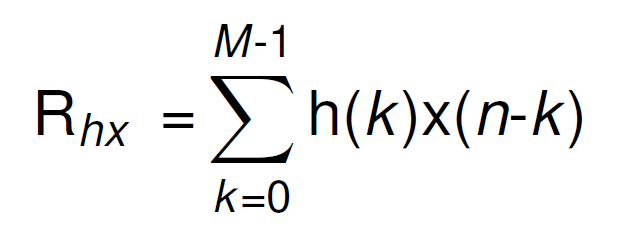
\includegraphics[width=6.3cm]{korW.PNG}
 \vspace{-0.3cm}
 \label{Splot_indeks}
\end{figure}


\end{labeling}

%%%%%%%%%%%%%%%%%%%%%%%%INSTRUKCA OBSŁUGI%%%%%%%%%%%%%%%%%%%%%%%%%%%%%%%%%%%%%%%%%%%%

\subsection{Instrukcja obsługi aplikacji}
Aplikacja do generacji szumów zawiera interfejs graficzny, który służy do obsługi przez użytkownika. Wygląd został przedstawiony na poniższym rysunku.
\newpage
\begin{figure}[h!]
 \centering
 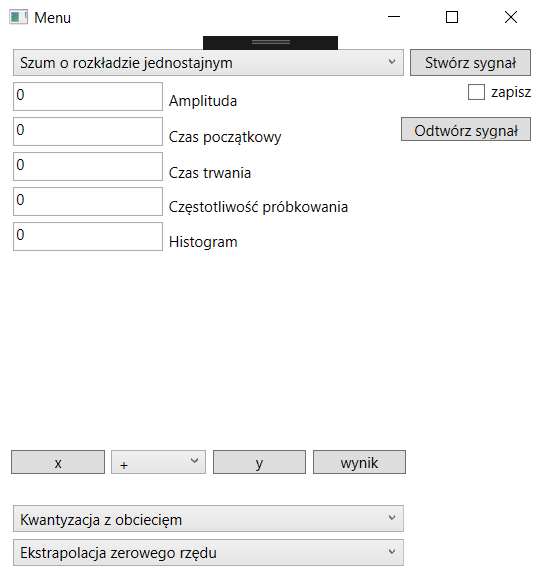
\includegraphics[width=9.3cm]{ui1.PNG}
 \vspace{-0.3cm}
 \caption{Widok główny aplikacji}
 \label{Widok_aplikacjis}
\end{figure}

Na górze okienka znajduje się wysuwana lista możliwych do generacji sygnałów. Obok znajduje się chceckbox, po zaznaczeniu którego sygnał zostanie zapisany do pliku.
Niżej jest przycisk do generacji sygnałów oraz lista parametrów wykresu. Tutaj wpisuje się dane wpływające na sygnał.
Pola umożliwiają ustawienie charakterystycznych parametrów sygnału. Na ich podstawie program wylicza wartości amplitudy sygnału w określonym czasie oraz wyświetla graficzną reprezentację sygnału w postaci wykresu funkcji amplitudy od czasu i histogramu.\\

Na dole okienka znajdują się przyciski: do odtwarzania sygnału z pliku, oraz do operacji na dwóch sygnałach. Po kliknięciu w x i y wybieramy odpowiednio pierwszy i dugi składnik działania. Między nimi można wybrać jedno z czterech działań.  Po wcisnięciu przycisku "wynik" program liczy wynik działania i wywietla jego graficzną reprezentację. 

\subsubsection{Generowanie sygnału}
Aby wygenerować sygnał użytkownik musi kliknąć w generuj sygnał.
\\Po wygenerowaniu sygnału pojawiają się dwa dodatkowe okienka aplikacji.
\begin{figure}[h!]
 \centering
 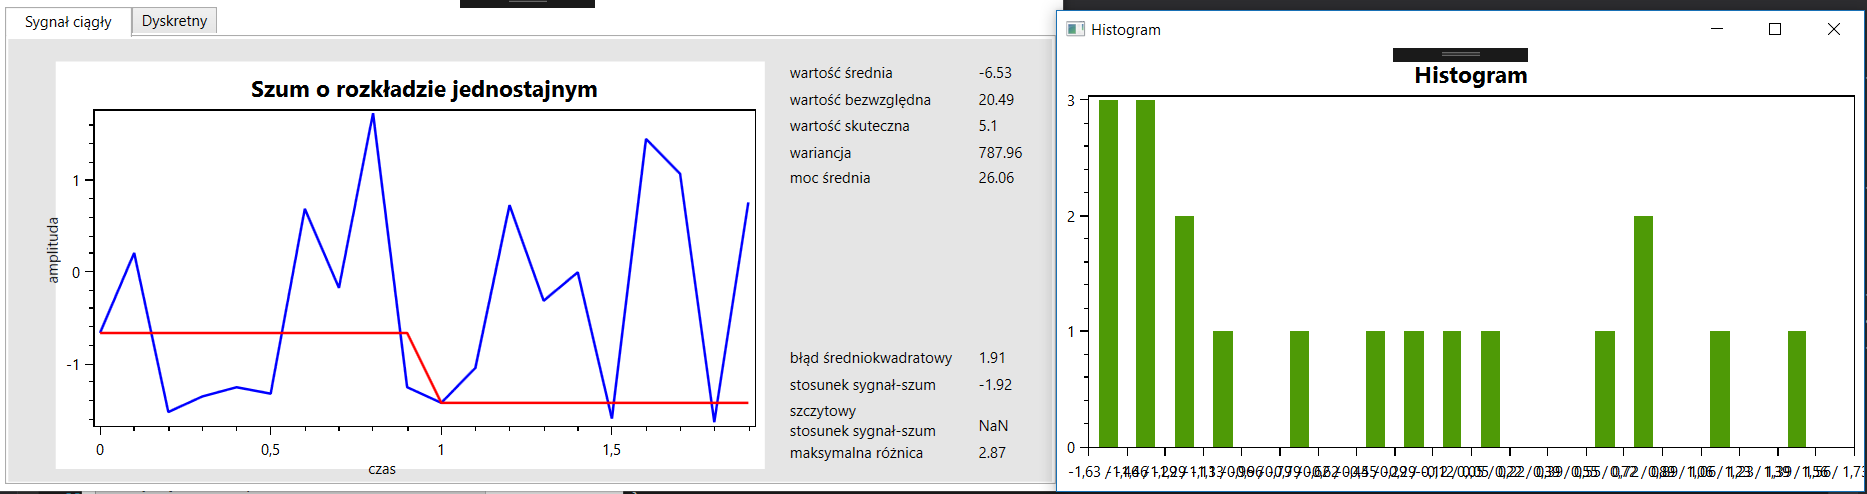
\includegraphics[width=15.3cm]{okienka.PNG}
 \vspace{-0.3cm}
 \caption{Okna po generacji sygnału}
 \label{Widok_aplikacjis}
\end{figure}
\\Jedno wyświetla histogram sygnału
\\Drugie przedstawia wykres funkcji amplitudy od czasu oraz obliczone wartości: wartość średnią, wartość średnią bezwzględną, wartość skuteczną, wariancję oraz moc średnią.

\subsubsection{Odczyt sygnału z pliku}
Oprócz generacji i zapisu do pliku, program umożliwia odczyt z pliku sygnału będącego wynikiem dyskretyzacji (bez kwantyzacji) wygenerowanego
sygnału ciągłego oraz sygnału będącego wynikiem operacji na dwóch sygnałach dyskretnych.
\\Tak jak w przypadku generacji, sygnał jest  reprezentowany graficznie w postaci histogramu i wykresu funkcji.

\subsection{Opis implementacji}
Aplikacja została napisana w wysokopoziomowym języku programowania - C\#. Do rysowania wykresów została wykorzystana zewnątrzna biblioteka OxyPlot. Program został napisany przy pomocy metodyki obiektowej i stosuje metody numeryczne.

\section{Eksperymenty i wyniki}

Poniżej znajdują się wszystkie przeprowadzone eksperymenty - możliwe do uzyskania w aplikacji sygnaly i wyniki. 

%%%%%%%%%%%%%%%%%%%%%%%%%%%%%%%%%%%%%%%%%%%%%%%%%%%%%%%%%%%%%%%%%%%%%%%%%%%%%%%%%%%%%%%%%%%%%%%%%%%%%%%%%%%%%%%%%
% PODROZDZIA PT. EKSPERYMENT NR 1 
%%%%%%%%%%%%%%%%%%%%%%%%%%%%%%%%%%%%%%%%%%%%%%%%%%%%%%%%%%%%%%%%%%%%%%%%%%%%%%%%%%%%%%%%%%%%%%%%%%%%%%%%%%%%%%%%%

\subsection{Eksperyment nr 1}

Eksperyment nr 1 -  Splot\\


\subsubsection{Założenia}
Operacja splotu jest przeprowadzana dla dwóch dowolnych sygnałów dyskretnych o wczeniej podanych (niekonieczcnie jednakowych) ilosciach próbek. W tym celu jest wykorzystany wzór \ref{Splot_indeks}.

\subsubsection{Przebieg}
Do generacji synału zostały podane parametry:
\addtokomafont{labelinglabel}{\sffamily}

\begin{labeling}{szj}
\item [Sygnał 1:]
\subitem [Amplituda (A):] 1
\subitem [Czas trwania (t1):] 5 s
\subitem [Częstotliwość próbkowania (d): ] 10 Hz
\subitem [Okres podstawowy :] 2 s

\begin{figure}[h!]
 \centering
 \includegraphics[width=12.3cm]{sin.PNG}
 \vspace{-0.3cm}
 \caption{Wykres sygnału sinusoidalnego}
 \label{sin}
\end{figure}

\item [Sygnał 2:]
\subitem [Amplituda (A):] 1
\subitem [Czas trwania (t1):] 5 s
\subitem [Częstotliwość próbkowania (d): ] 10 Hz

\end{labeling}

\begin{figure}[h!]
 \centering
 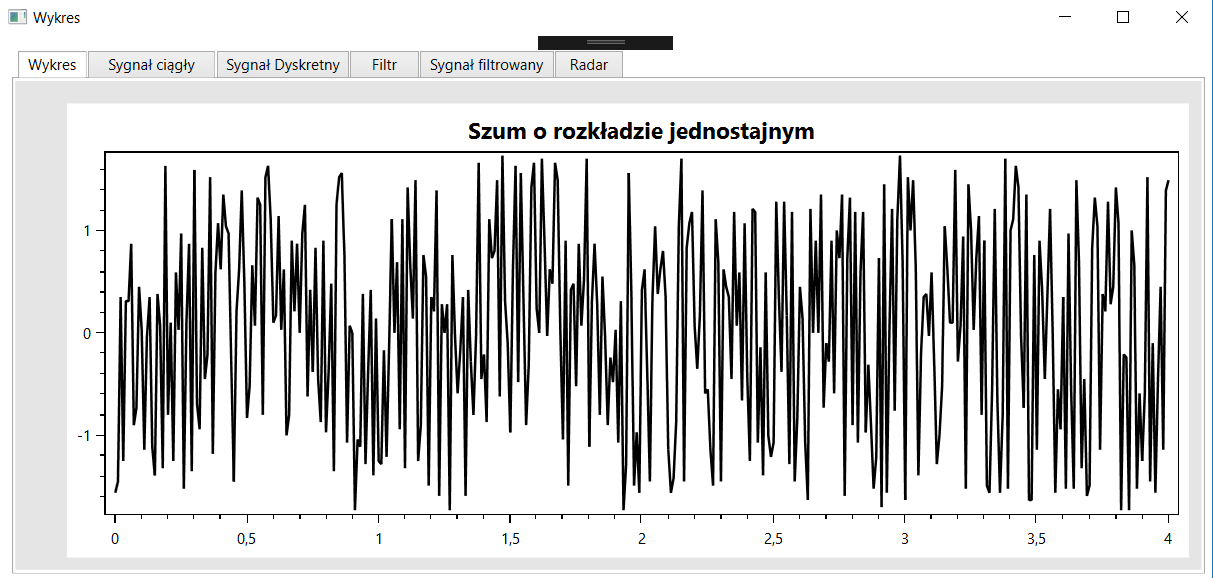
\includegraphics[width=12.3cm]{szum.PNG}
 \vspace{-0.3cm}
 \caption{Wykres szumu gausowskiego}
 \label{szum}
\end{figure}
 \newpage
\subsubsection{Rezultat}

Rezultat przedstawia zamieszczony poniżej zrzut ekranu z programu. Wartości liczbowe oraz wykres funkcji amplitudy od czasu przedstawia \ref{Wykres dla wynikw eksperymentu pierwszego}.
\begin{figure}[h!]
 \centering
 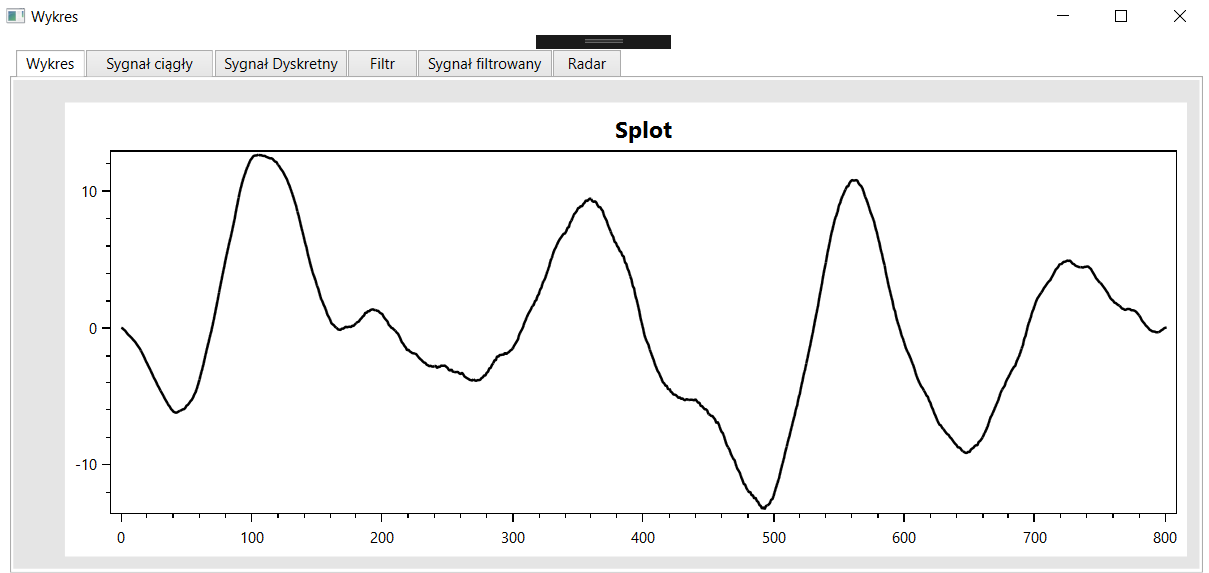
\includegraphics[width=12.3cm]{splot.PNG}
 \vspace{-0.3cm}
 \caption{Wykres splotu sygnałów 1 i 2}
 \label{Wykres dla wynikw eksperymentu pierwszego}
\end{figure}


%%%%%%%%%%%%%%%%%%%%%%%%%%%%%%%%%%%%%%%%%%%%%%%%%%%%%%%%%%%%%%%%%%%%%%%%%%%%%%%%%%%%%%%%%%%%%%%%%%%%%%%%%%%%%%%%%
% PODROZDZIA PT. EKSPERYMENT NR2 
%%%%%%%%%%%%%%%%%%%%%%%%%%%%%%%%%%%%%%%%%%%%%%%%%%%%%%%%%%%%%%%%%%%%%%%%%%%%%%%%%%%%%%%%%%%%%%%%%%%%%%%%%%%%%%%%%

\subsection{Eksperyment nr 2}
10 20
Eksperyment nr 2  - Filtracja z filtrem dolnoprzepustowym
\subsubsection{Założenia}
Filtr dolnoprzepustowy opisuje wzór, na podstawie odwrotnego przekształcenia Fouriera:

\begin{figure}[h!]
 \centering
 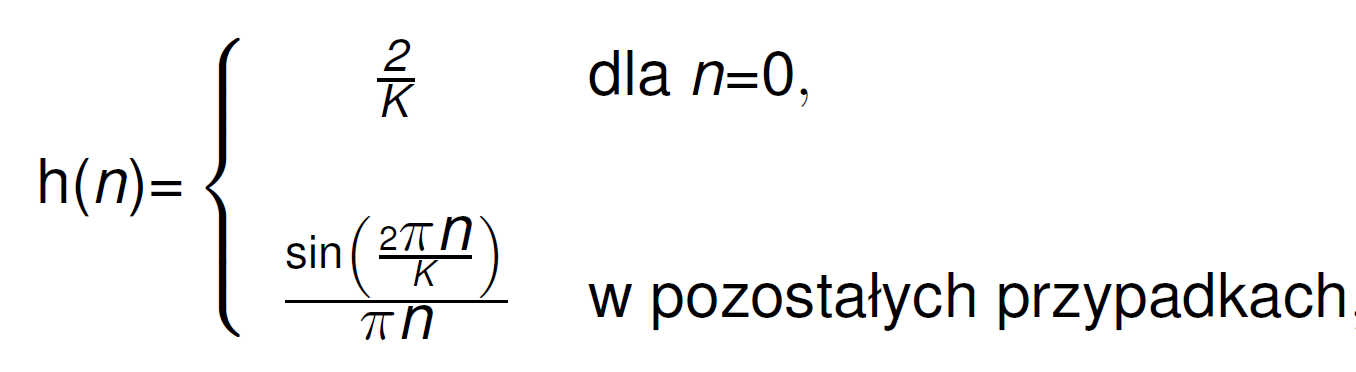
\includegraphics[width=4.3cm]{four.PNG}
 \vspace{-0.3cm}
 \label{gw}
\end{figure}

gdzie:
\subitem n - liczba całkowita,
\subitem częstotliwosć odcięcia filtru - f0 =  fp/K

Zakładamy, że filtr jest idealny -  w pasmie przepustowym nie zmienia się widmo sygnału wejsciowego -  transmitancja jest równa  1. W pasmie zaporowym skłądowe czętotliwosciowe zostaną kompletnie wytłumione (transmitancja równa 0).

Ze względu na nieskońconą liczbę współczynników h(n) nie stosuje się tego wzoru w praktyce.

Wzór na odpowiedź impulsową filtru o M współczynników z przesunięciem (w celu uzyskania nieujemnych indeksów):

\begin{figure}[h!]
 \centering
 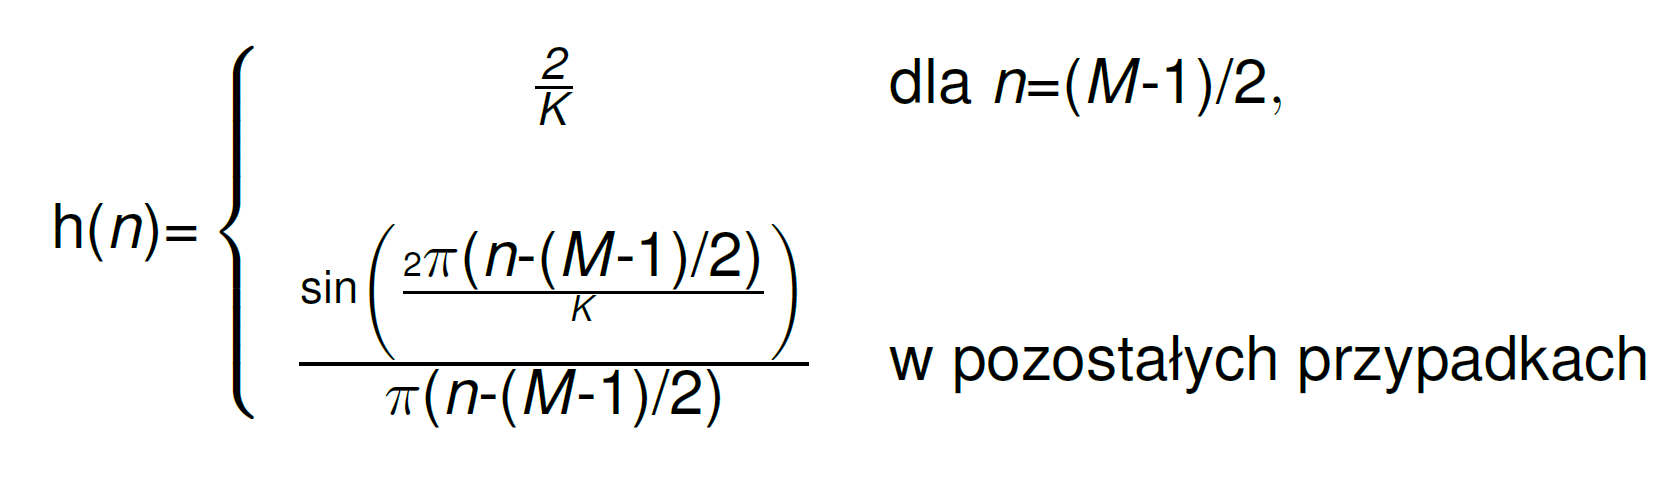
\includegraphics[width=4.3cm]{f.PNG}
 \vspace{-0.3cm}
 \label{gw}
\end{figure}

gdzie:
\subitem n = 0,1, ... , M-1
\subitem częstotliwosć odcięcia filtru - f0 =  fp/K

\subsubsection{Przebieg}
Do generacji synału prostokątnego zostały podane parametry:
\addtokomafont{labelinglabel}{\sffamily}

\begin{labeling}{szj}
\item [Amplituda (A):] 1
\item [Czas trwania (t1):] 100 s
\item [Częstotliwość próbkowania (d): ] 1 Hz
\item [Okres podstawowy :] 100 s
\item [Współczynnik wypełnienia:] 0,5
\end{labeling}

Wykres sygnału przedstawia poniższy obrazek:
\begin{figure}[h!]
 \centering
 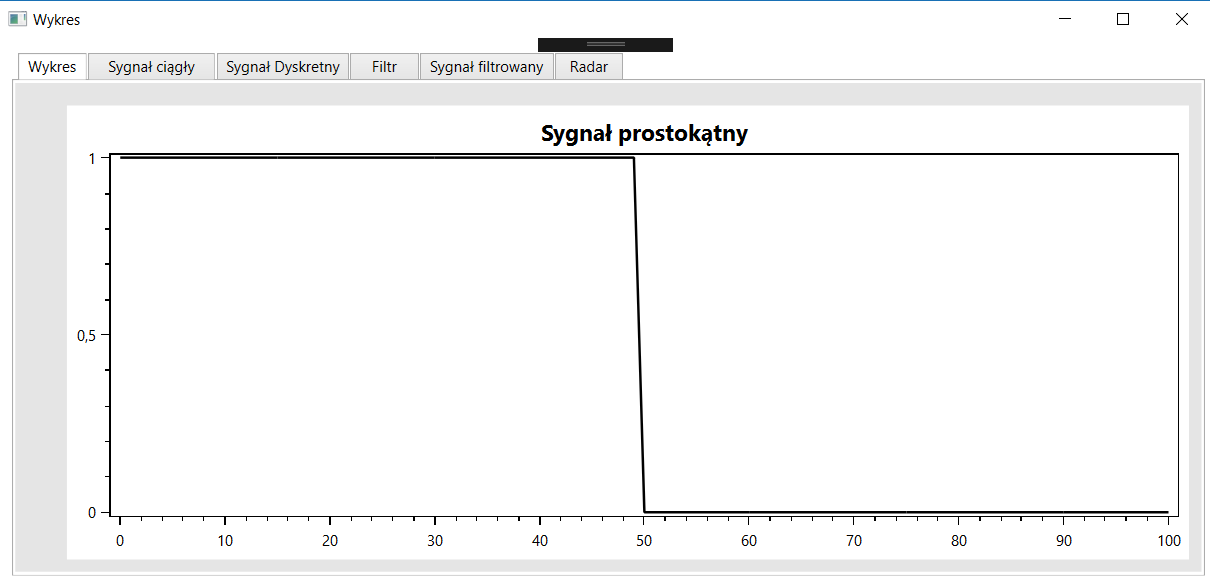
\includegraphics[width=12.3cm]{prost.PNG}
 \vspace{-0.3cm}
 \label{gw}
\end{figure}

Parametry filtracji:
\addtokomafont{labelinglabel}{\sffamily}

\begin{labeling}{szj}
\item [K:] 10
\item [M:] 20 
\end{labeling}

\subsubsection{Rezultat}

Rezultaty przedstawiają zamieszczone poniżej zrzuty ekranu z programu. 
\newpage
Okno prostokątne
\begin{figure}[h!]
 \centering
 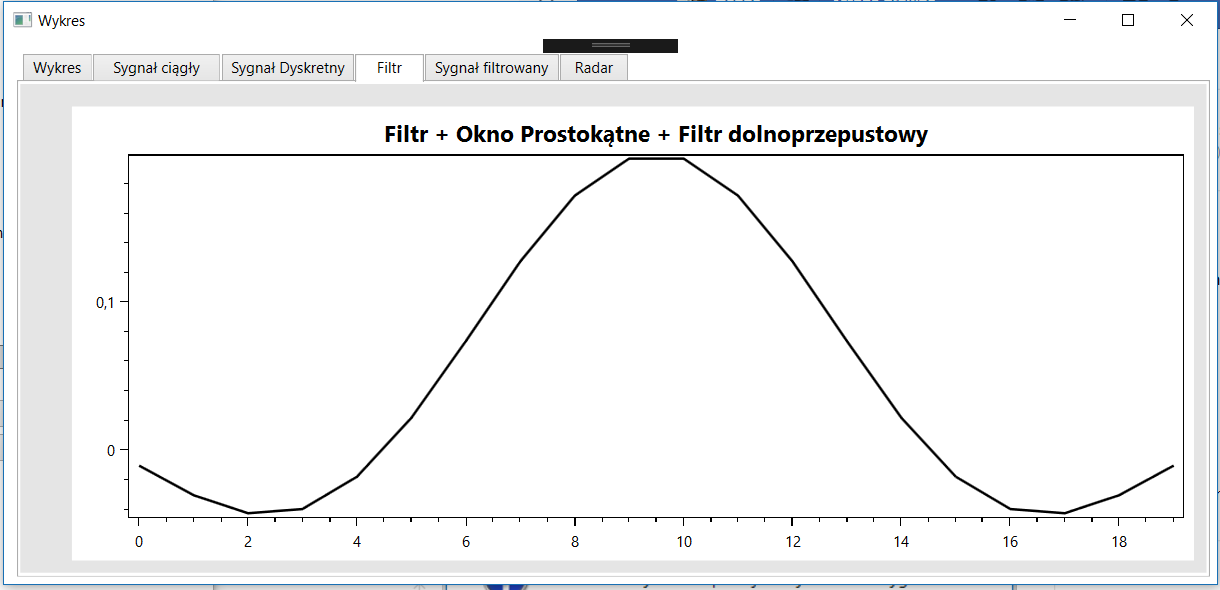
\includegraphics[width=12.3cm]{prostFDOP.PNG}
 \vspace{-0.3cm}
 \caption{Filtracja dolnoprzepustowa z oknem prostokątnym}
 \label{Wykres dla wyników eksperymentu drugiego}
\end{figure}
\newpage
Rys. \ref{Wykres dla wynikw eksperymentu pierwszego h} przedstawia histogram sygnału z opisanymi powyżej parametrami. 
\begin{figure}[h!]
 \centering
 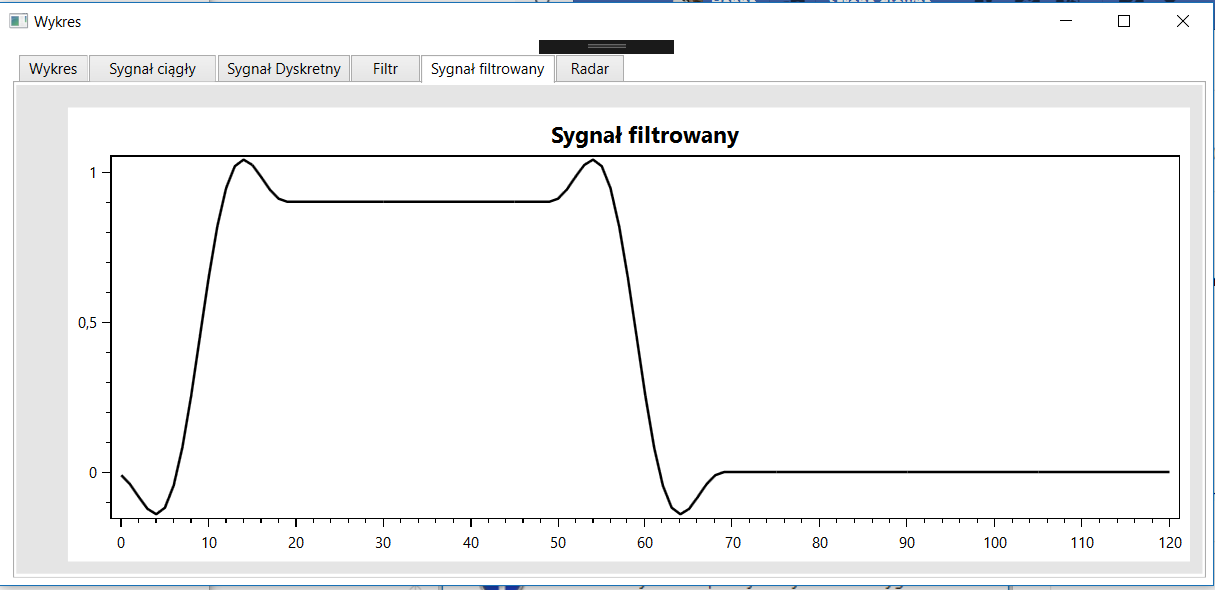
\includegraphics[width=12.3cm]{prostSFDP.PNG}
 \vspace{-0.3cm}
 \caption{Sygnał filtracja dolnoprzepustowej z oknem prostokątnym}
 \label{Histogram dla wyników eksperymentu drugiego}
\end{figure}

\newpage
Okno Hamminga
\begin{figure}[h!]
 \centering
 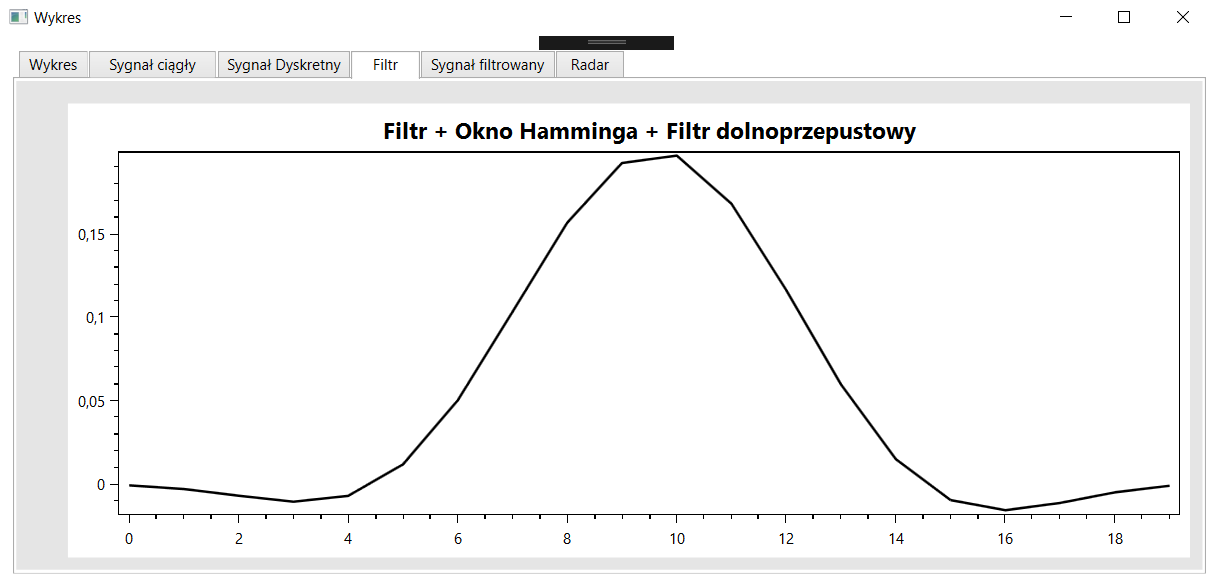
\includegraphics[width=12.3cm]{prostFDOHm.PNG}
 \vspace{-0.3cm}
 \caption{Filtracja dolnoprzepustowa z oknem Hamminga}
 \label{Wykres dla wyników eksperymentu drugiego}
\end{figure}
\newpage
Rys. \ref{Wykres dla wynikw eksperymentu pierwszego h} przedstawia histogram sygnału z opisanymi powyżej parametrami. 
\begin{figure}[h!]
 \centering
 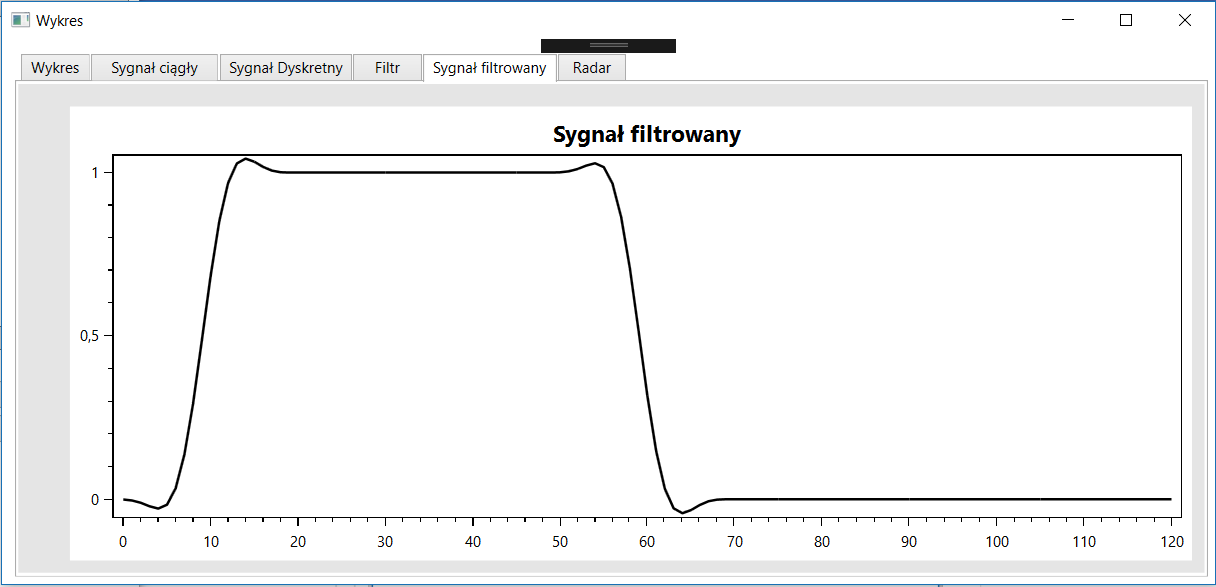
\includegraphics[width=12.3cm]{prostSFDHm.PNG}
 \vspace{-0.3cm}
 \caption{Sygnał filtracja dolnoprzepustowej z oknem Hamminga}
 \label{Histogram dla wyników eksperymentu drugiego}
\end{figure}

\newpage
Okno Hanninga
\begin{figure}[h!]
 \centering
 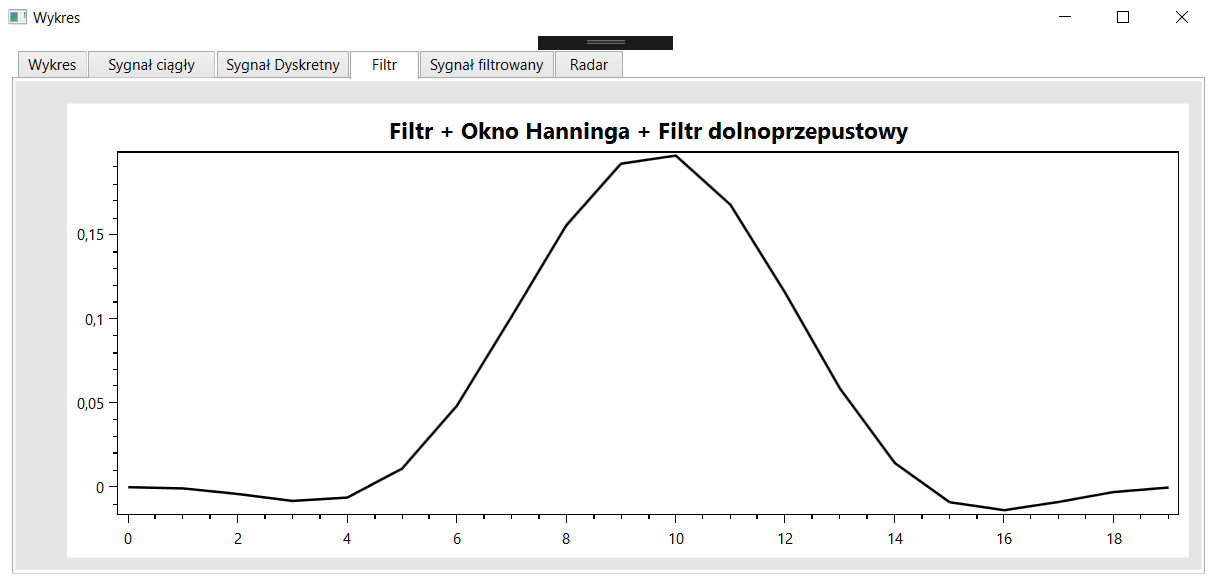
\includegraphics[width=12.3cm]{prostFDOHn.PNG}
 \vspace{-0.3cm}
 \caption{Filtracja dolnoprzepustowa z oknem Hanninga}
 \label{Wykres dla wyników eksperymentu drugiego}
\end{figure}
\newpage
Rys. \ref{Wykres dla wynikw eksperymentu pierwszego h} przedstawia histogram sygnału z opisanymi powyżej parametrami. 
\begin{figure}[h!]
 \centering
 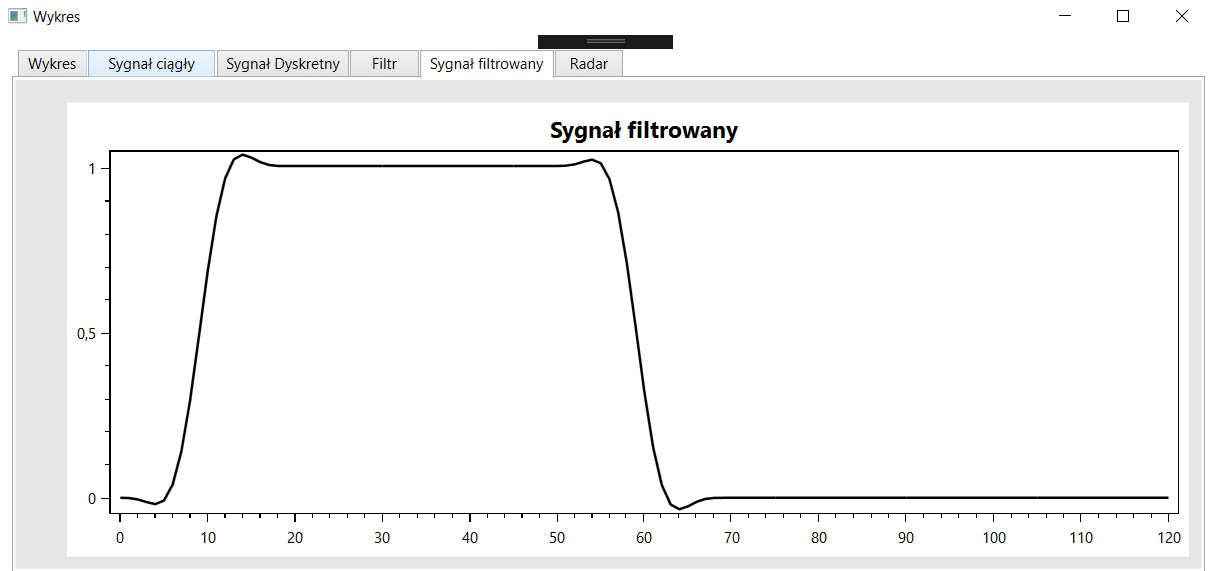
\includegraphics[width=12.3cm]{prostSFDHn.PNG}
 \vspace{-0.3cm}
 \caption{Sygnał filtracji dolnoprzepustowej z oknem Hanninga}
 \label{Histogram dla wyników eksperymentu drugiego}
\end{figure}

\newpage
Okno Blackmana
\begin{figure}[h!]
 \centering
 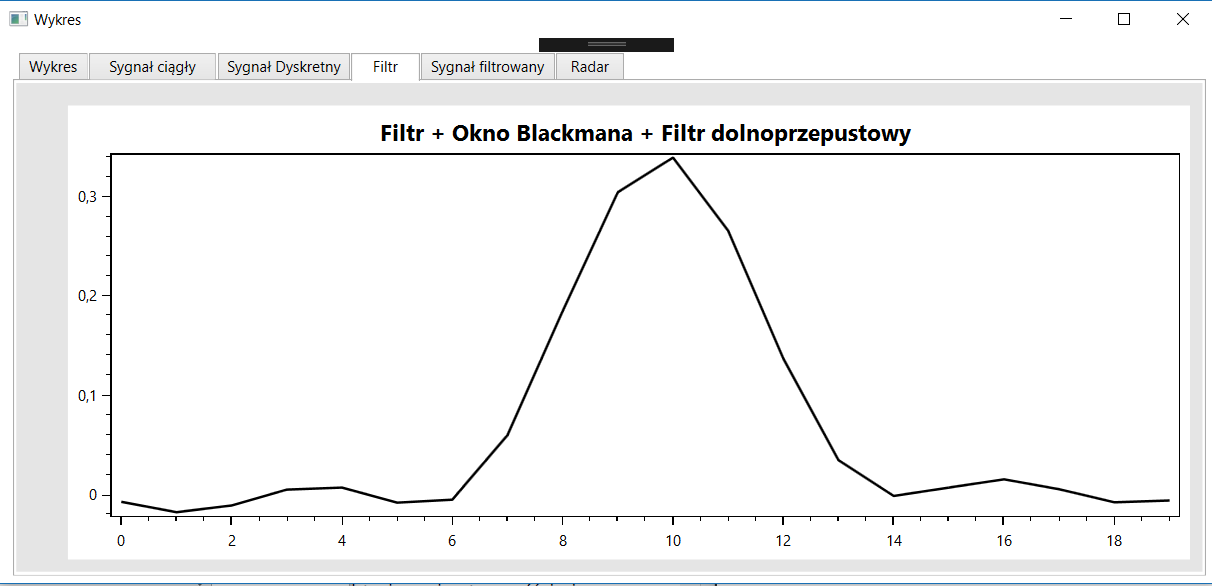
\includegraphics[width=12.3cm]{prostFDOB.PNG}
 \vspace{-0.3cm}
 \caption{Filtracja dolnoprzepustowa z oknem Blackmana}
 \label{Wykres dla wyników eksperymentu drugiego}
\end{figure}
\newpage
Rys. \ref{Wykres dla wynikw eksperymentu pierwszego h} przedstawia histogram sygnału z opisanymi powyżej parametrami. 
\begin{figure}[h!]
 \centering
 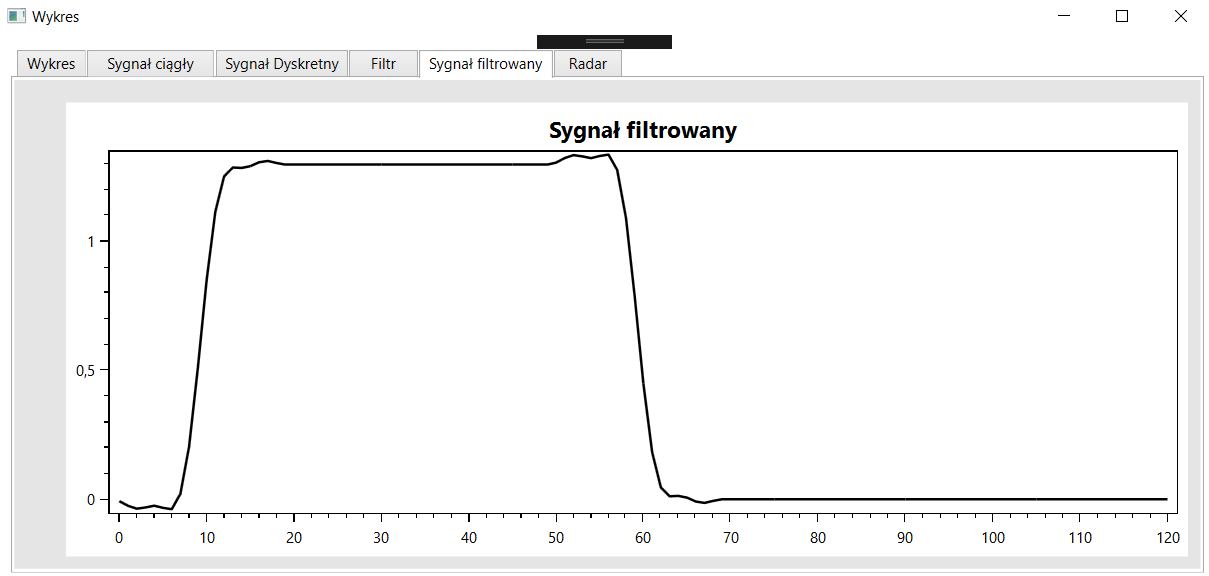
\includegraphics[width=12.3cm]{prostSFDB.PNG}
 \vspace{-0.3cm}
 \caption{Sygnał filtracji dolnoprzepustowej z oknem Blackmana}
 \label{Histogram dla wyników eksperymentu drugiego}
\end{figure}

%%%%%%%%%%%%%%%%%%%%%%%%%%%%%%%%%%%%%%%%%%%%%%%%%%%%%%%%%%%%%%%%%%%%%%%%%%%%%%%%%%%%%%%%%%%%%%%%%%%%%%%%%%%%%%%%%
% PODROZDZIA PT. EKSPERYMENT NR 3
%%%%%%%%%%%%%%%%%%%%%%%%%%%%%%%%%%%%%%%%%%%%%%%%%%%%%%%%%%%%%%%%%%%%%%%%%%%%%%%%%%%%%%%%%%%%%%%%%%%%%%%%%%%%%%%%%

\subsection{Eksperyment nr 3}

Eksperyment nr 3  - Filtracja z filtrem srodkowoprzepustowym
\subsubsection{Założenia}
Z wykorzystaniem twierdzenia o modulacji przekształcamy odpowiedź impulsową filtru dolnoprzepustowego do odpowiedzi filtru srodkowoprzepustowego:
współczynniki h(n) są mnożone przez sygnał sinusoidalny  o częstotliwosci f = fp/4

Wtedy fd = fp/4-f0 i fg = fp/4 + f0.

\subsubsection{Przebieg}
Do generacji synału prostokątnego zostały podane parametry:
\addtokomafont{labelinglabel}{\sffamily}

\begin{labeling}{szj}
\item [Amplituda (A):] 1
\item [Czas trwania (t1):] 100 s
\item [Częstotliwość próbkowania (d): ] 1 Hz
\item [Okres podstawowy :] 100 s
\item [Współczynnik wypełnienia:] 0,5
\end{labeling}

Wykres sygnału przedstawia poniższy obrazek:
\begin{figure}[h!]
 \centering
 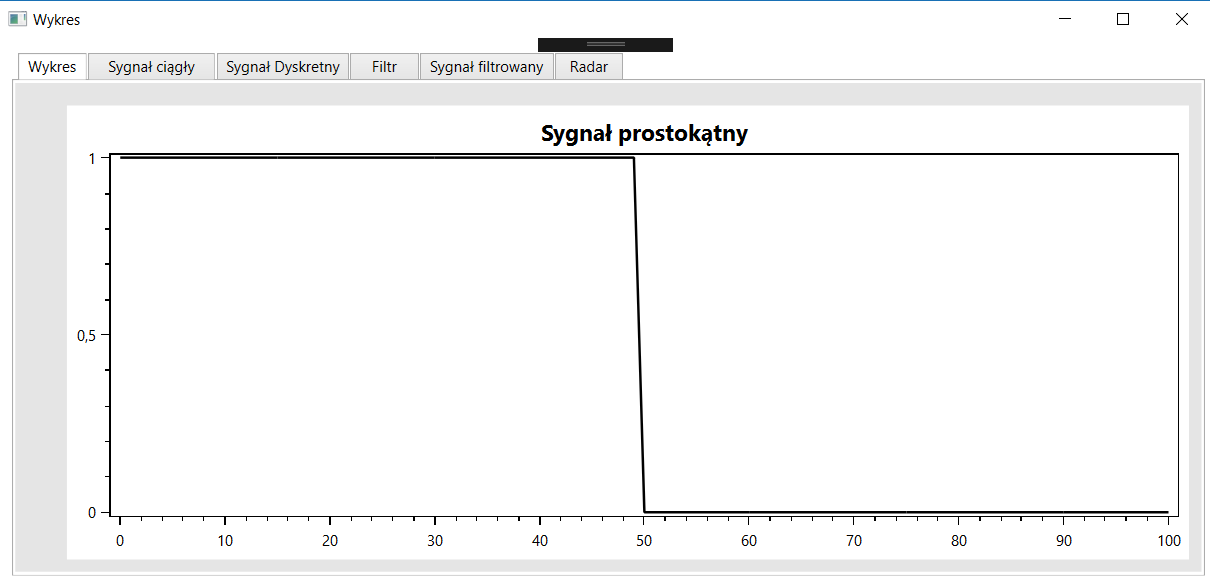
\includegraphics[width=12.3cm]{prost.PNG}
 \vspace{-0.3cm}
 \label{gw}
\end{figure}

Parametry filtracji:
\addtokomafont{labelinglabel}{\sffamily}

\begin{labeling}{szj}
\item K:] 10
\item [M:] 20 s
\end{labeling}

\subsubsection{Rezultat}

Rezultaty przedstawiają zamieszczone poniżej zrzuty ekranu z programu. 
\newpage
Okno prostokątne
\begin{figure}[h!]
 \centering
 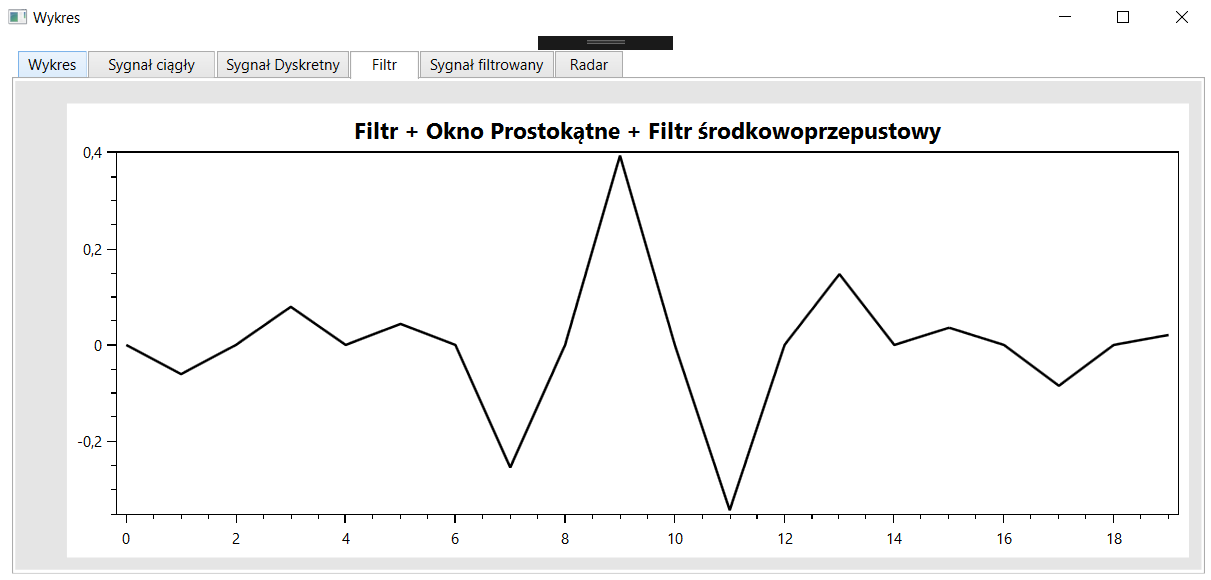
\includegraphics[width=12.3cm]{prostFSOP.PNG}
 \vspace{-0.3cm}
 \caption{Filtracja srodkowoprzepustowa z oknem prostokątnym}
 \label{Wykres dla wyników eksperymentu drugiego}
\end{figure}
\newpage
Rys. \ref{Wykres dla wynikw eksperymentu pierwszego h} przedstawia histogram sygnału z opisanymi powyżej parametrami. 
\begin{figure}[h!]
 \centering
 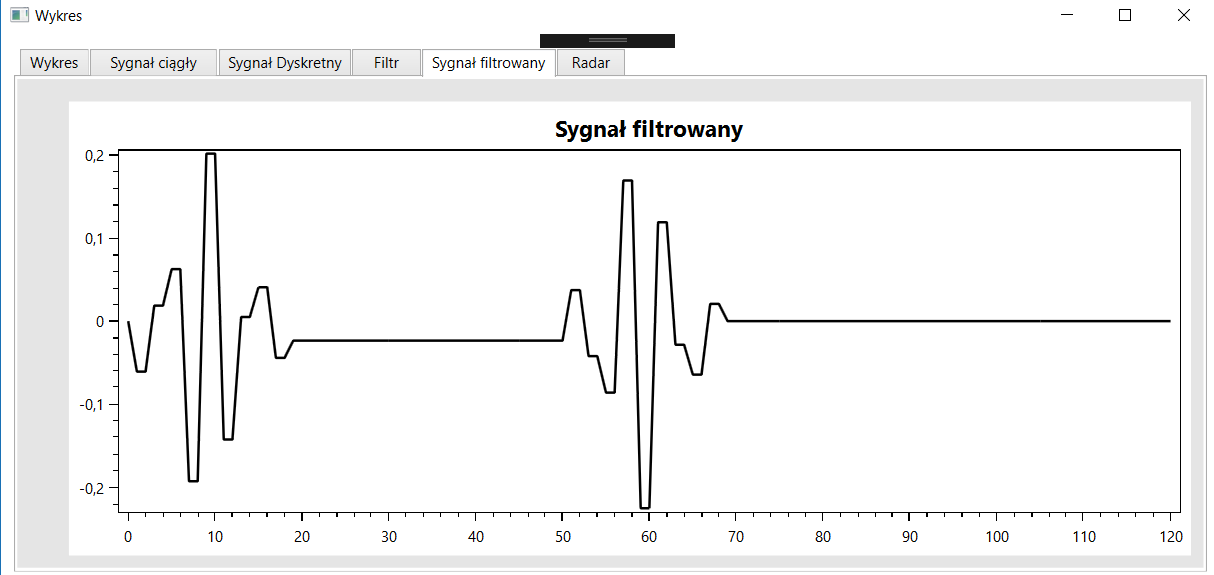
\includegraphics[width=12.3cm]{prostSFSP.PNG}
 \vspace{-0.3cm}
 \caption{Sygnał filtracji srodkowoprzepustowej z oknem prostokątnym}
 \label{Histogram dla wyników eksperymentu drugiego}
\end{figure}

\newpage
Okno Hamminga
\begin{figure}[h!]
 \centering
 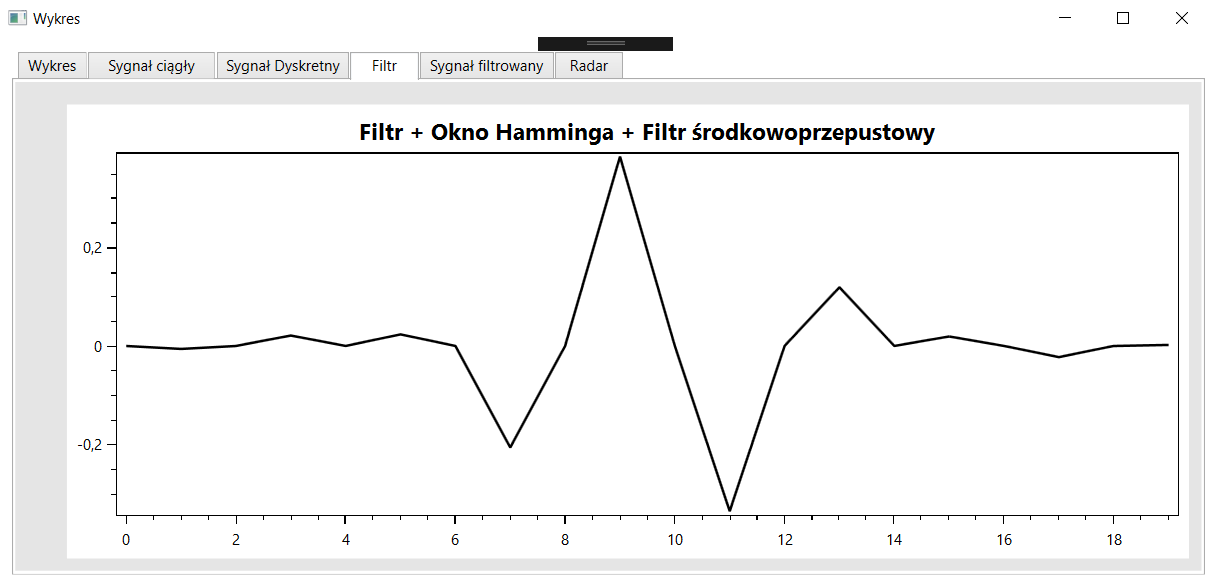
\includegraphics[width=12.3cm]{prostFSOHm.PNG}
 \vspace{-0.3cm}
 \caption{Filtracja srodkowoprzepustowa z oknem Hamminga}
 \label{Wykres dla wyników eksperymentu drugiego}
\end{figure}
\newpage
Rys. \ref{Wykres dla wynikw eksperymentu pierwszego h} przedstawia histogram sygnału z opisanymi powyżej parametrami. 
\begin{figure}[h!]
 \centering
 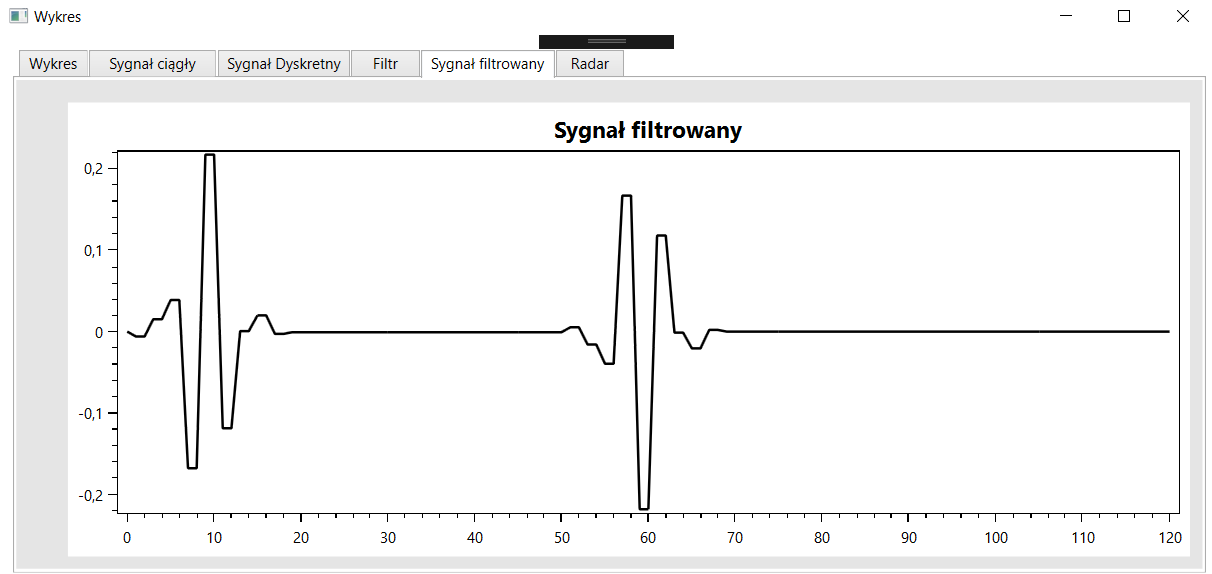
\includegraphics[width=12.3cm]{prostSFSHm.PNG}
 \vspace{-0.3cm}
 \caption{Sygnał filtracji srodkowoprzepustowej z oknem Hamminga}
 \label{Histogram dla wyników eksperymentu drugiego}
\end{figure}

\newpage
Okno Hanninga
\begin{figure}[h!]
 \centering
 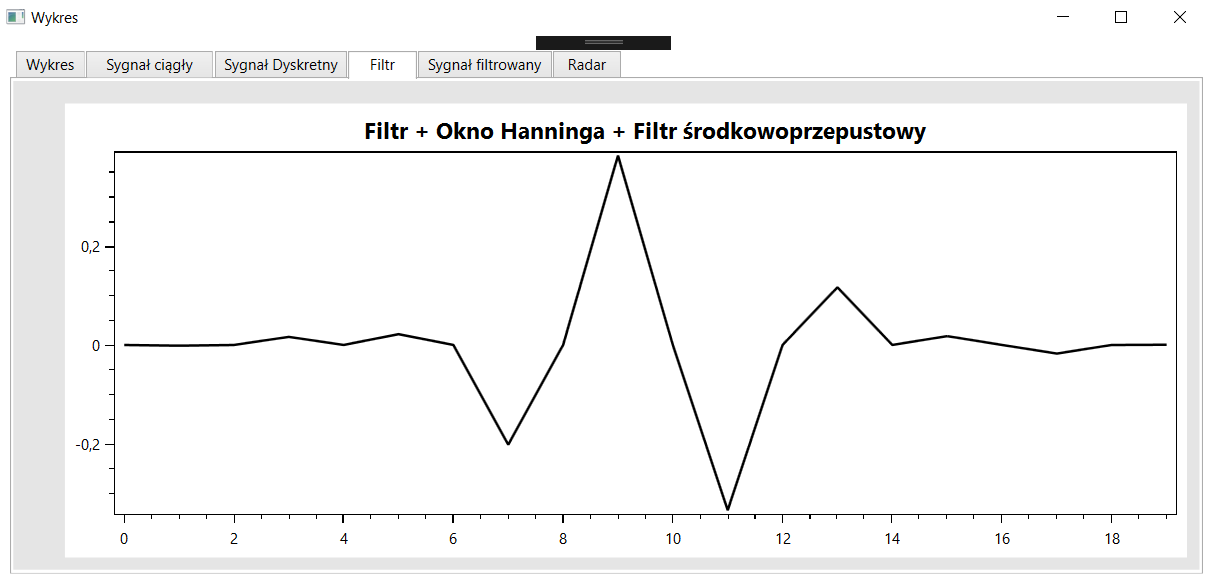
\includegraphics[width=12.3cm]{prostFSOHn.PNG}
 \vspace{-0.3cm}
 \caption{Filtracja srodkowoprzepustowa z oknem prostokątnym}
 \label{Wykres dla wyników eksperymentu drugiego}
\end{figure}
\newpage
Rys. \ref{Wykres dla wynikw eksperymentu pierwszego h} przedstawia histogram sygnału z opisanymi powyżej parametrami. 
\begin{figure}[h!]
 \centering
 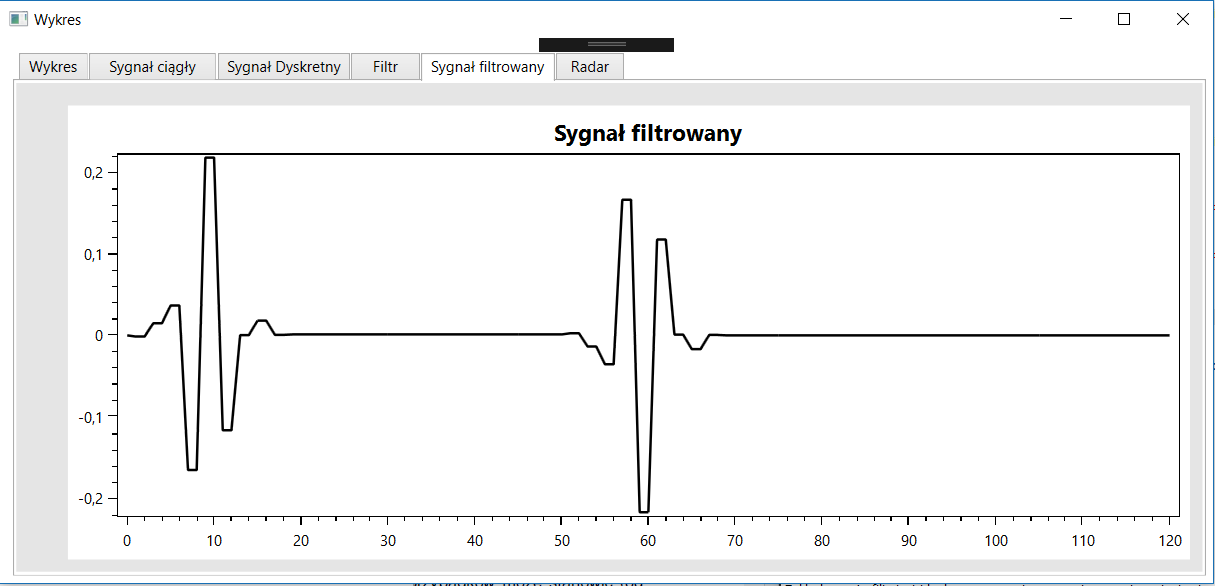
\includegraphics[width=12.3cm]{prostSFSHn.PNG}
 \vspace{-0.3cm}
 \caption{Sygnał filtracji srodkowoprzepustowej z oknem Hamminga}
 \label{Histogram dla wyników eksperymentu drugiego}
\end{figure}

\newpage
Okno Blackmana
\begin{figure}[h!]
 \centering
 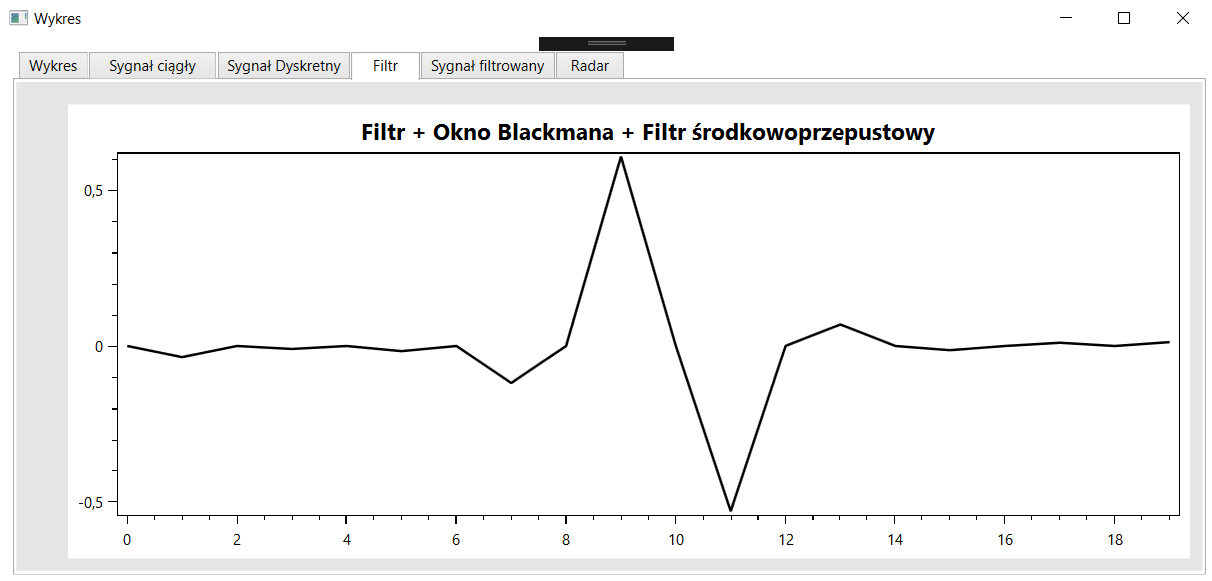
\includegraphics[width=12.3cm]{prostFSOB.PNG}
 \vspace{-0.3cm}
 \caption{Filtracja srodkowoprzepustowa z oknem prostokątnym}
 \label{Wykres dla wyników eksperymentu drugiego}
\end{figure}
\newpage
Rys. \ref{Wykres dla wynikw eksperymentu pierwszego h} przedstawia histogram sygnału z opisanymi powyżej parametrami. 
\begin{figure}[h!]
 \centering
 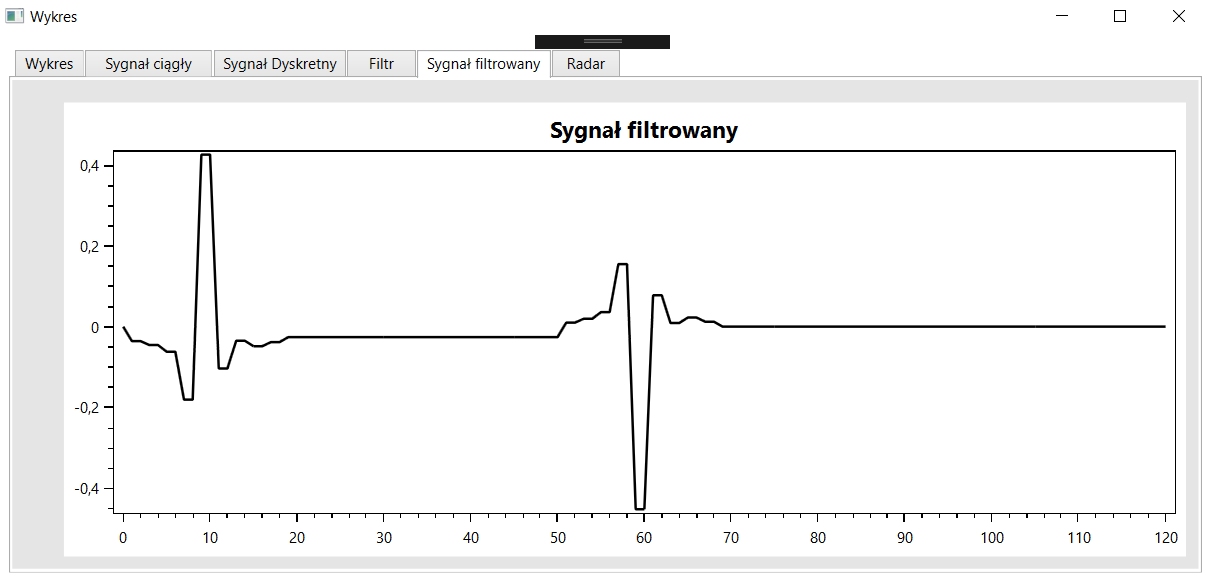
\includegraphics[width=12.3cm]{prostSFSB.PNG}
 \vspace{-0.3cm}
 \caption{Sygnał filtracji srodkowoprzepustowej z oknem Hamminga}
 \label{Histogram dla wyników eksperymentu drugiego}
\end{figure}


%%%%%%%%%%%%%%%%%%%%%%%%%%%%%%%%%%%%%%%%%%%%%%%%%%%%%%%%%%%%%%%%%%%%%%%%%%%%%%%%%%%%%%%%%%%%%%%%%%%%%%%%%%%%%%%%%
% PODROZDZIA PT. EKSPERYMENT NR 4 
%%%%%%%%%%%%%%%%%%%%%%%%%%%%%%%%%%%%%%%%%%%%%%%%%%%%%%%%%%%%%%%%%%%%%%%%%%%%%%%%%%%%%%%%%%%%%%%%%%%%%%%%%%%%%%%%%

\subsection{Eksperyment nr 4}

Eksperyment nr 4  - Filtracja z filtrem górnoprzepustowym
\subsubsection{Założenia}
Z wykorzystaniem twierdzenia o modulacji przekształcamy odpowiedź impulsową filtru dolnoprzepustowego do odpowiedzi filtru górnoprzepustowego:
współczynniki h(n) są mnożone przez sygnał sinusoidalny  o częstotliwosci f = fp/2. Wtedy f0 = fp/2-f0 (f0 -  nowa częstotliwosć odcięcia).

\subsubsection{Przebieg}
Do generacji synału prostokątnego zostały podane parametry:
\addtokomafont{labelinglabel}{\sffamily}

\begin{labeling}{szj}
\item [Amplituda (A):] 1
\item [Czas trwania (t1):] 100 s
\item [Częstotliwość próbkowania (d): ] 1 Hz
\item [Okres podstawowy :] 100 s
\item [Współczynnik wypełnienia:] 0,5
\end{labeling}

Wykres sygnału przedstawia poniższy obrazek:
\begin{figure}[h!]
 \centering
 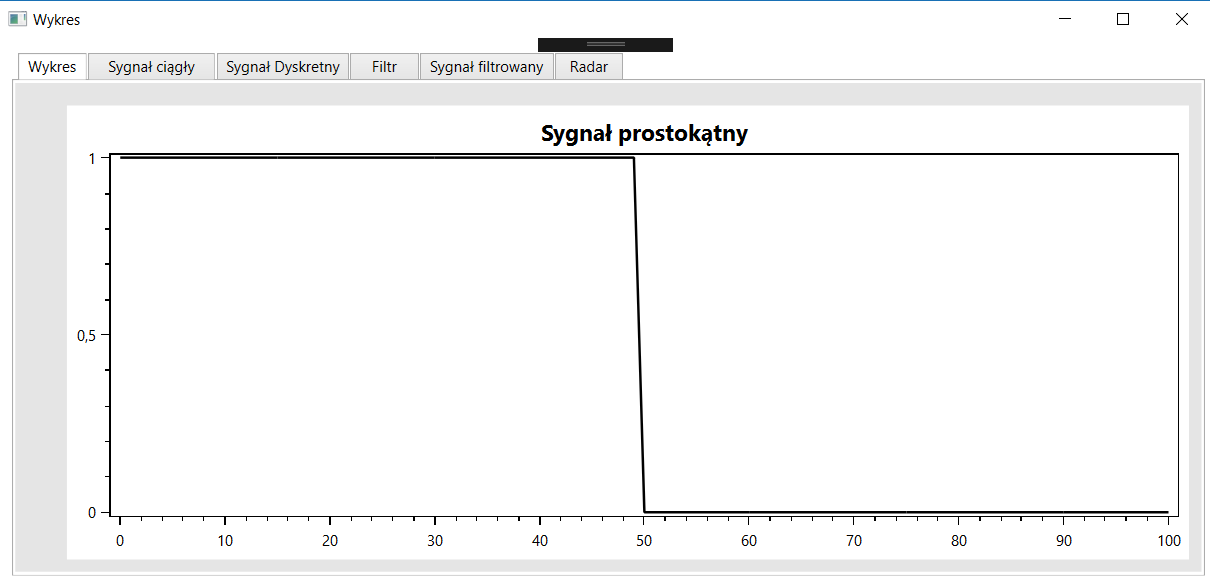
\includegraphics[width=12.3cm]{prost.PNG}
 \vspace{-0.3cm}
 \label{gw}
\end{figure}

Parametry filtracji:
\addtokomafont{labelinglabel}{\sffamily}

\begin{labeling}{szj}
\item K:] 10
\item [M:] 20 s
\end{labeling}

\subsubsection{Rezultat}

Rezultaty przedstawiają zamieszczone poniżej zrzuty ekranu z programu. 
\newpage
Okno prostokątne
\begin{figure}[h!]
 \centering
 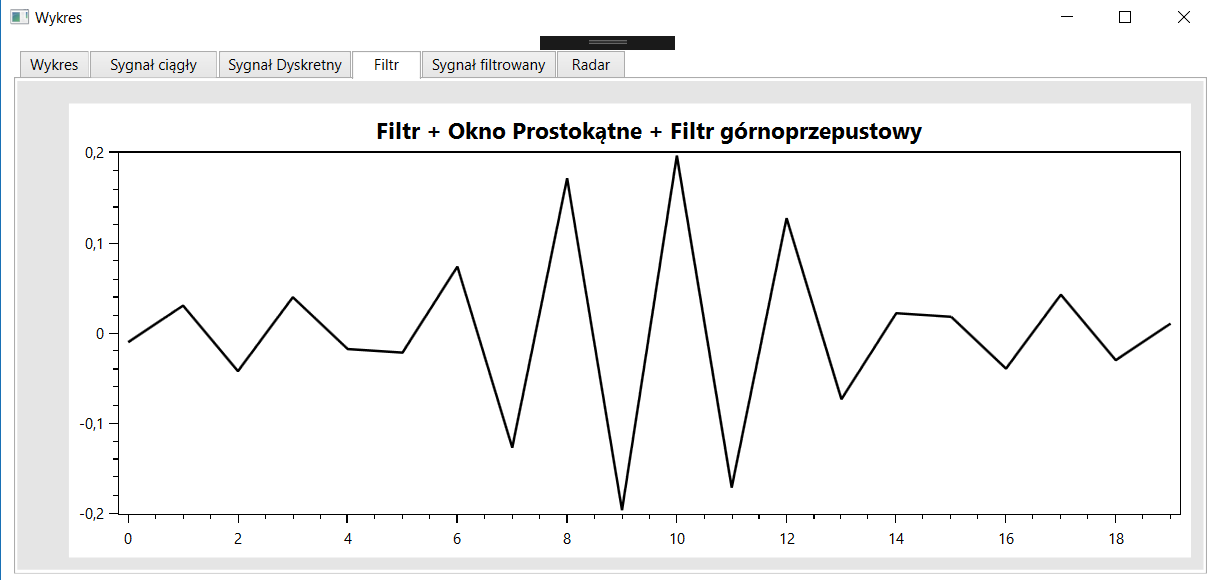
\includegraphics[width=12.3cm]{prostFGOP.PNG}
 \vspace{-0.3cm}
 \caption{Filtracja górnoprzepustowa z oknem prostokątnym}
 \label{Wykres dla wyników eksperymentu drugiego}
\end{figure}
\newpage
Rys. \ref{Wykres dla wynikw eksperymentu pierwszego h} przedstawia histogram sygnału z opisanymi powyżej parametrami. 
\begin{figure}[h!]
 \centering
 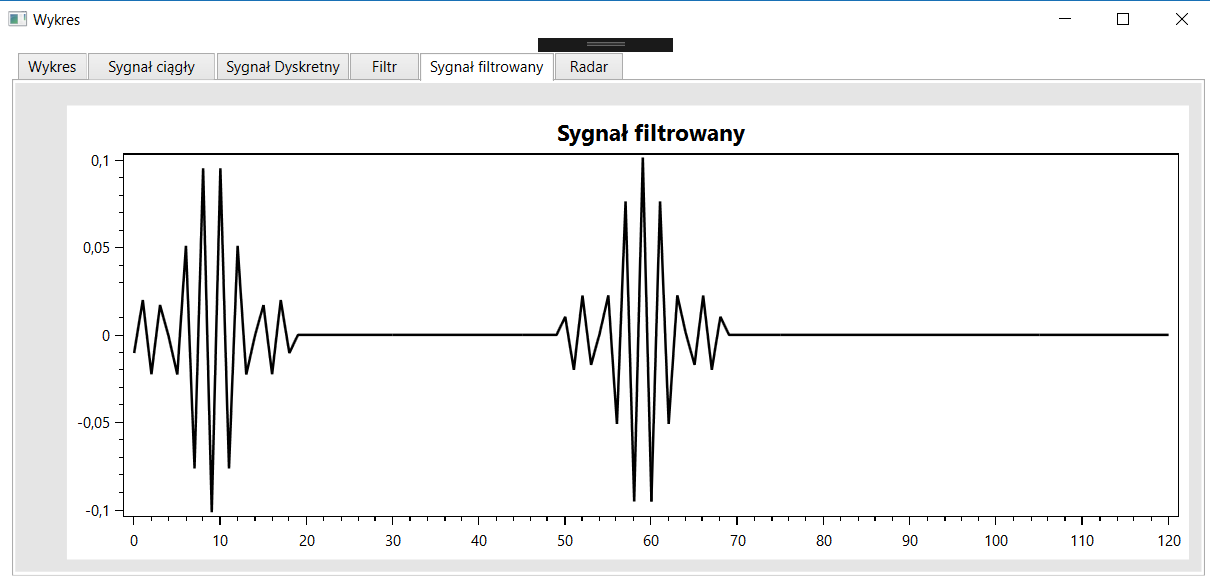
\includegraphics[width=12.3cm]{prostSFGP.PNG}
 \vspace{-0.3cm}
 \caption{Sygnał filtracji górnoprzepustowej z oknem prostokątnym}
 \label{Histogram dla wyników eksperymentu drugiego}
\end{figure}

\newpage
Okno Hamminga
\begin{figure}[h!]
 \centering
 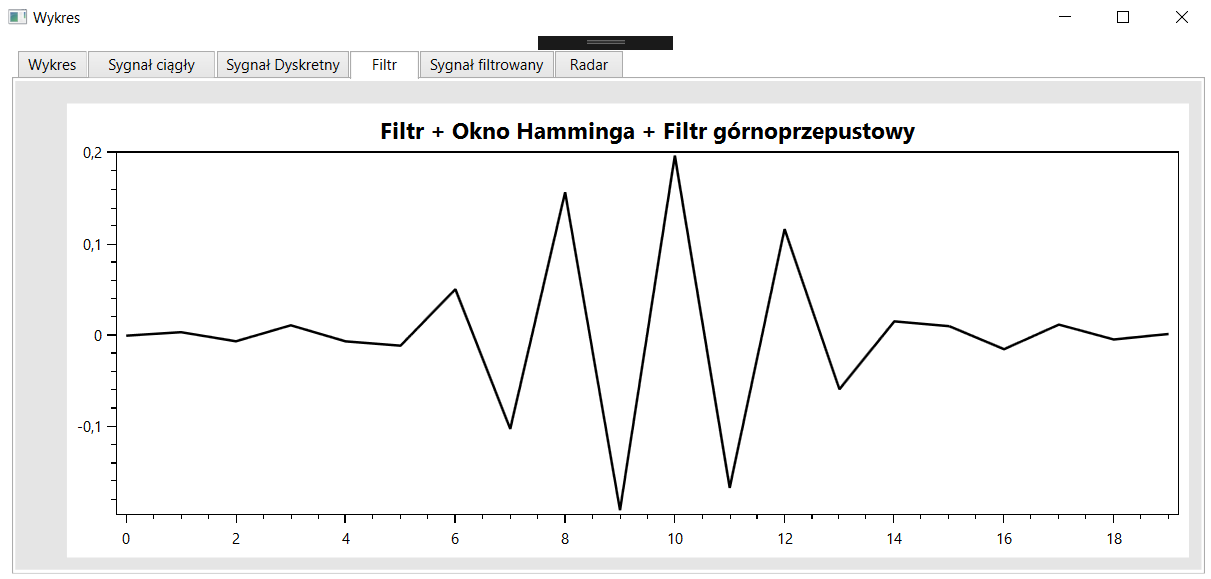
\includegraphics[width=12.3cm]{prostFGOHm.PNG}
 \vspace{-0.3cm}
 \caption{Filtracja górnoprzepustowa z oknem Hamminga}
 \label{Wykres dla wyników eksperymentu drugiego}
\end{figure}
\newpage
Rys. \ref{Wykres dla wynikw eksperymentu pierwszego h} przedstawia histogram sygnału z opisanymi powyżej parametrami. 
\begin{figure}[h!]
 \centering
 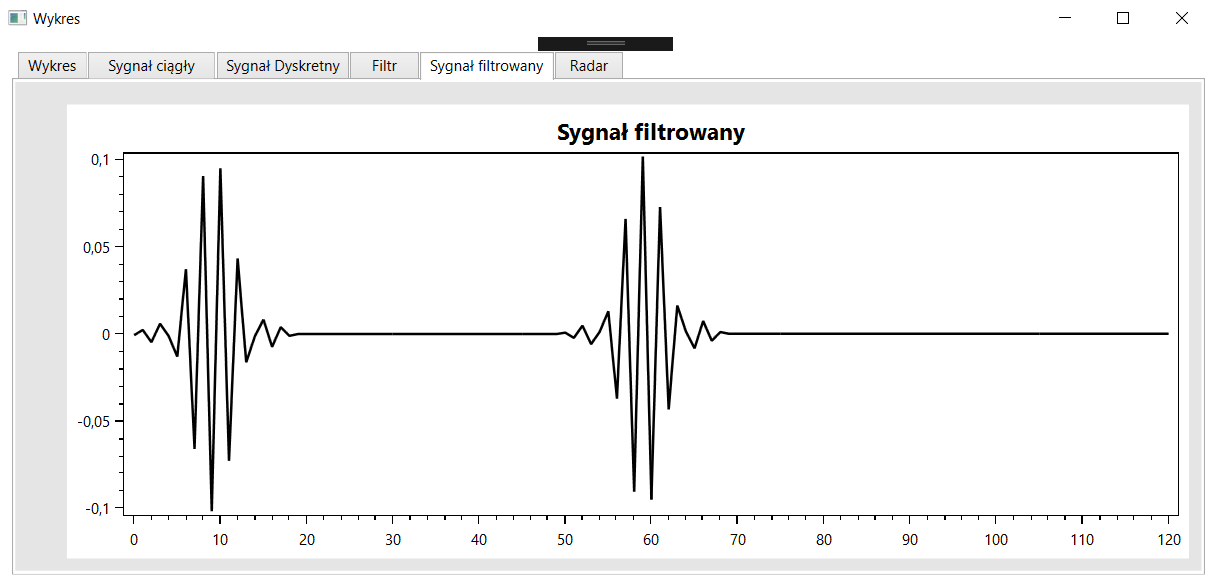
\includegraphics[width=12.3cm]{prostSFGHm.PNG}
 \vspace{-0.3cm}
 \caption{Sygnał filtracji górnoprzepustowej z oknem Hamminga}
 \label{Histogram dla wyników eksperymentu drugiego}
\end{figure}

\newpage
Okno Hanninga
\begin{figure}[h!]
 \centering
 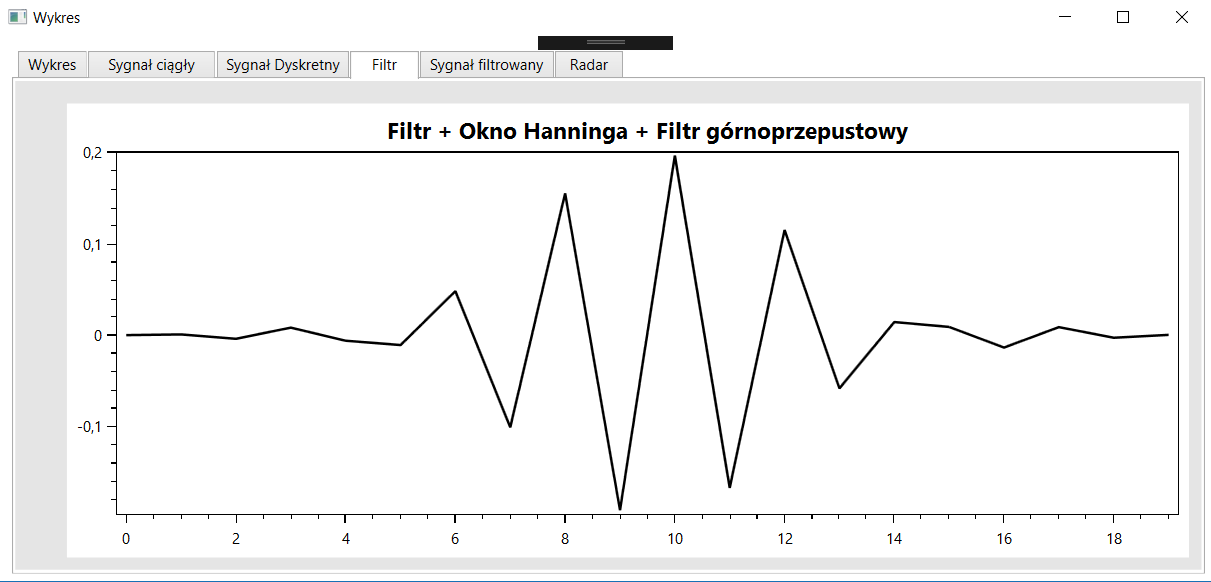
\includegraphics[width=12.3cm]{prostFGOHn.PNG}
 \vspace{-0.3cm}
 \caption{Filtracja górnoprzepustowa z oknem Hanninga}
 \label{Wykres dla wyników eksperymentu drugiego}
\end{figure}
\newpage
Rys. \ref{Wykres dla wynikw eksperymentu pierwszego h} przedstawia histogram sygnału z opisanymi powyżej parametrami. 
\begin{figure}[h!]
 \centering
 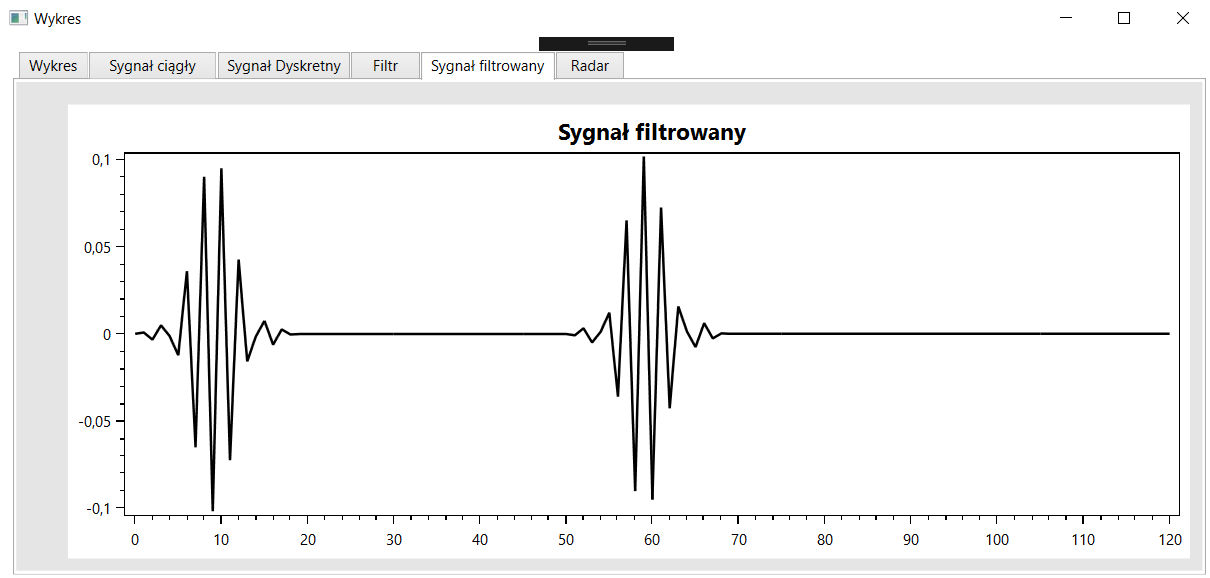
\includegraphics[width=12.3cm]{prostSFGHn.PNG}
 \vspace{-0.3cm}
 \caption{Sygnał filtracji górnoprzepustowej z oknem Hanninga}
 \label{Histogram dla wyników eksperymentu drugiego}
\end{figure}

\newpage
Okno Blackmana
\begin{figure}[h!]
 \centering
 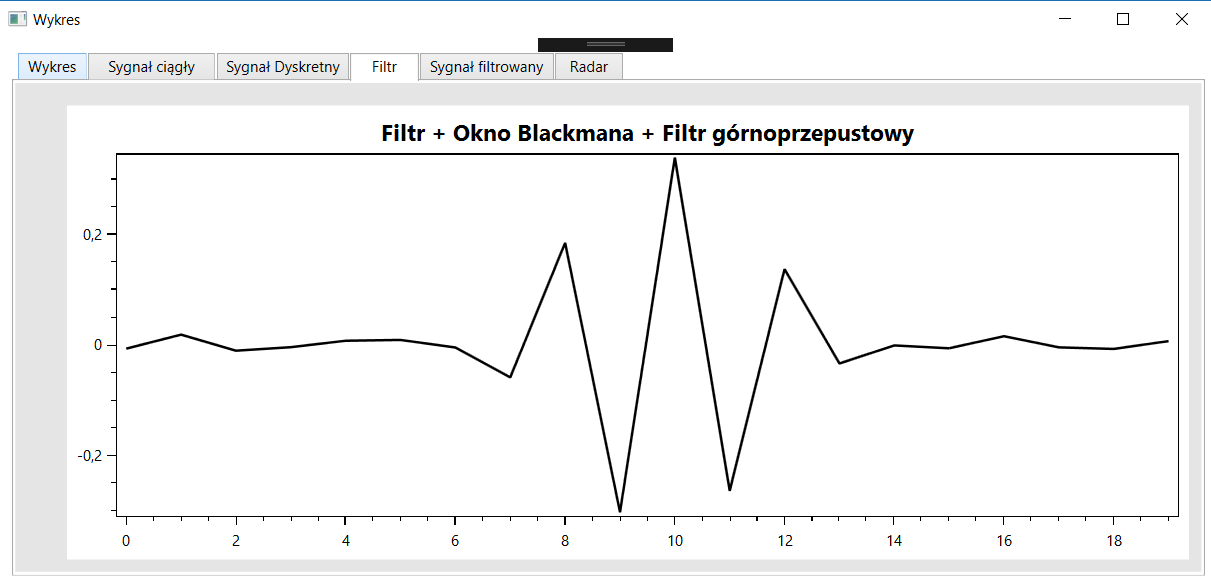
\includegraphics[width=12.3cm]{prostFGOB.PNG}
 \vspace{-0.3cm}
 \caption{Filtracja górnoprzepustowa z oknem Blackmana}
 \label{Wykres dla wyników eksperymentu drugiego}
\end{figure}
\newpage
Rys. \ref{Wykres dla wynikw eksperymentu pierwszego h} przedstawia histogram sygnału z opisanymi powyżej parametrami. 
\begin{figure}[h!]
 \centering
 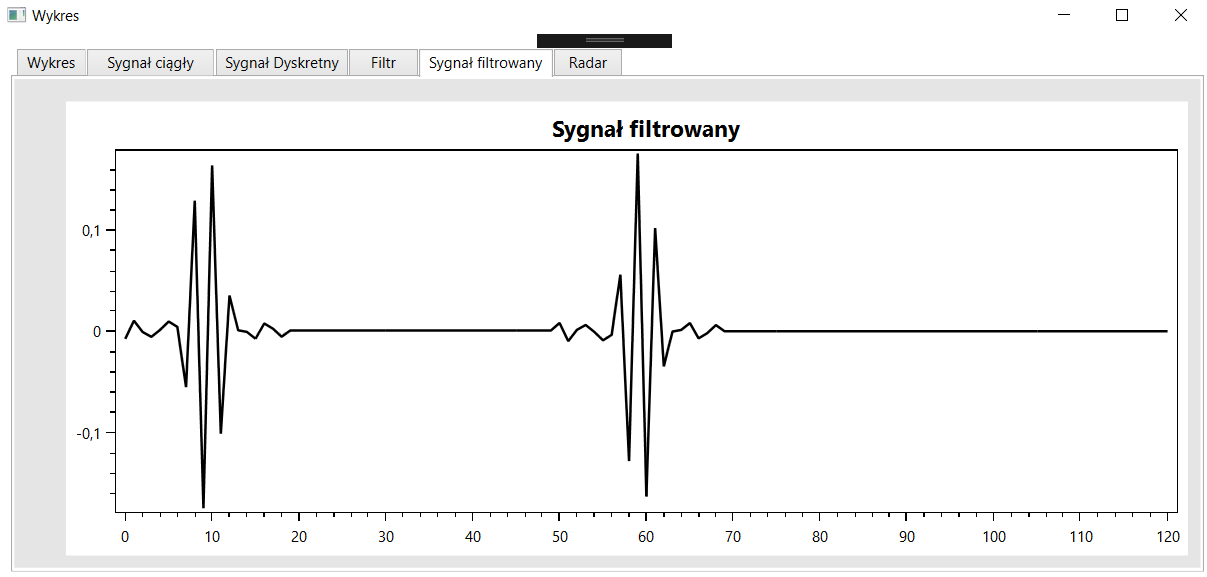
\includegraphics[width=12.3cm]{prostSFGB.PNG}
 \vspace{-0.3cm}
 \caption{Sygnał filtracji górnoprzepustowa z oknem Blackmana}
 \label{Histogram dla wyników eksperymentu drugiego}
\end{figure}


%%%%%%%%%%%%%%%%%%%%%%%%%%%%%%%%%%%%%%%%%%%%%%%%%%%%%%%%%%%%%%%%%%%%%%%%%%%%%%%%%%%%%%%%%%%%%%%%%%%%%%%%%%%%%%%%%
% PODROZDZIA PT. EKSPERYMENT NR 5
%%%%%%%%%%%%%%%%%%%%%%%%%%%%%%%%%%%%%%%%%%%%%%%%%%%%%%%%%%%%%%%%%%%%%%%%%%%%%%%%%%%%%%%%%%%%%%%%%%%%%%%%%%%%%%%%%

\subsection{Eksperyment nr 5}

Eksperyment nr 5 - Korelacja\\

\subsubsection{Założenia}
Operacja splotu jest przeprowadzana dla dwóch dowolnych sygnałów dyskretnych o wczeniej podanych (niekonieczcnie jednakowych) ilosciach próbek. W tym celu jest wykorzystany wzór \ref{Splot_indeks}.

\subsubsection{Przebieg}
Do generacji synału zostały podane parametry:
\addtokomafont{labelinglabel}{\sffamily}

\begin{labeling}{szj}
\item [Sygnał 1:]
\subitem [Amplituda (A):] 1
\subitem [Czas trwania (t1):] 5 s
\subitem [Częstotliwość próbkowania (d): ] 10 Hz
\subitem [Okres podstawowy :] 2 s

\begin{figure}[h!]
 \centering
 \includegraphics[width=12.3cm]{sin.PNG}
 \vspace{-0.3cm}
 \caption{Wykres sygnału sinusoidalnego}
 \label{sin}
\end{figure}

\item [Sygnał 2:]
\subitem [Amplituda (A):] 1
\subitem [Czas trwania (t1):] 5 s
\subitem [Częstotliwość próbkowania (d): ] 10 Hz

\end{labeling}

\begin{figure}[h!]
 \centering
 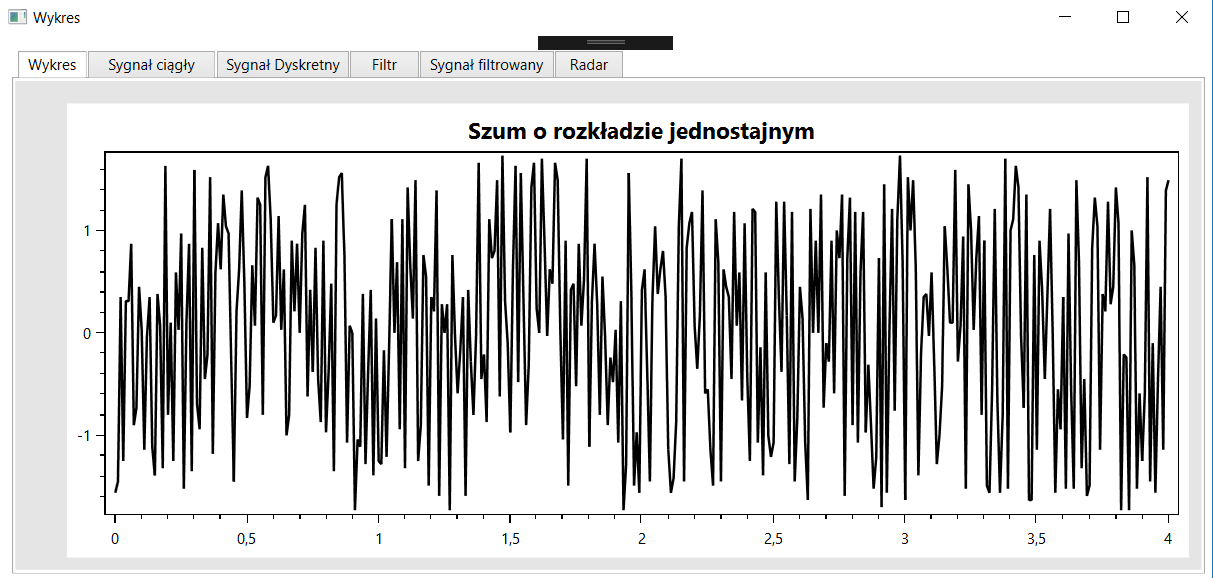
\includegraphics[width=12.3cm]{szum.PNG}
 \vspace{-0.3cm}
 \caption{Wykres szumu gausowskiego}
 \label{szum}
\end{figure}
 \newpage
\subsubsection{Rezultat}

Korelacja bezposrednia:
\\Rezultat przedstawia zamieszczony poniżej zrzut ekranu z programu. Wartości liczbowe oraz wykres funkcji amplitudy od czasu przedstawia \ref{Wykres dla wynikw eksperymentu pierwszego}.
\begin{figure}[h!]
 \centering
 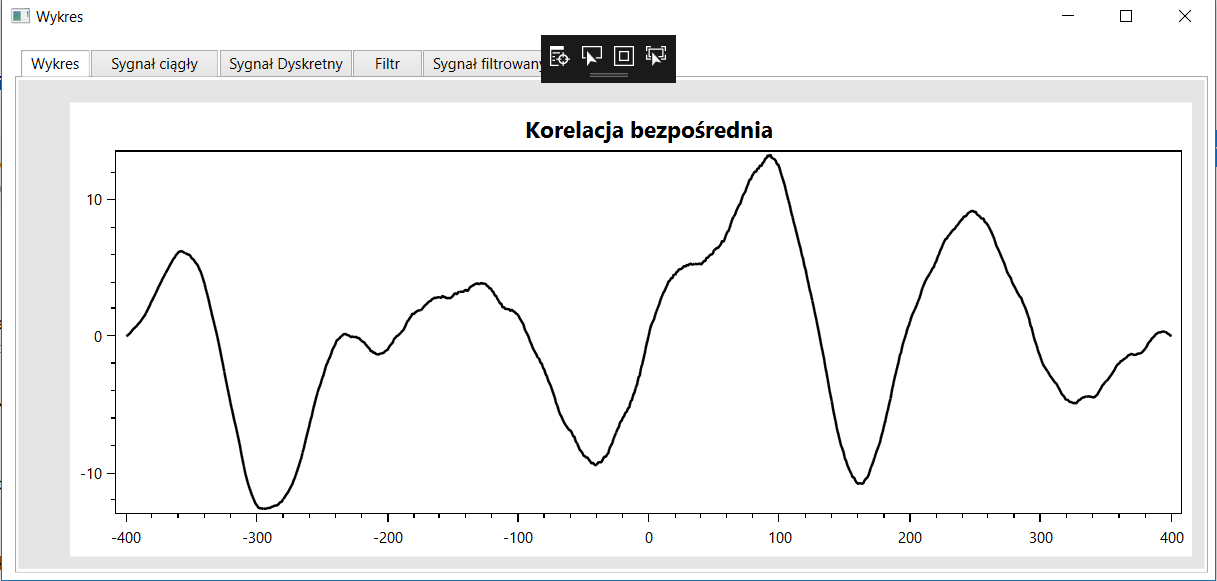
\includegraphics[width=12.3cm]{korB.PNG}
 \vspace{-0.3cm}
 \caption{Wykres sygnału sinusoidalnego ciągły: kwantyzacja z obcięciem, interpolacja pierwszego rzędu}
 \label{Wykres dla wynikw eksperymentu pierwszego}
\end{figure}
 \newpage
\begin{figure}[h!]
 \centering
 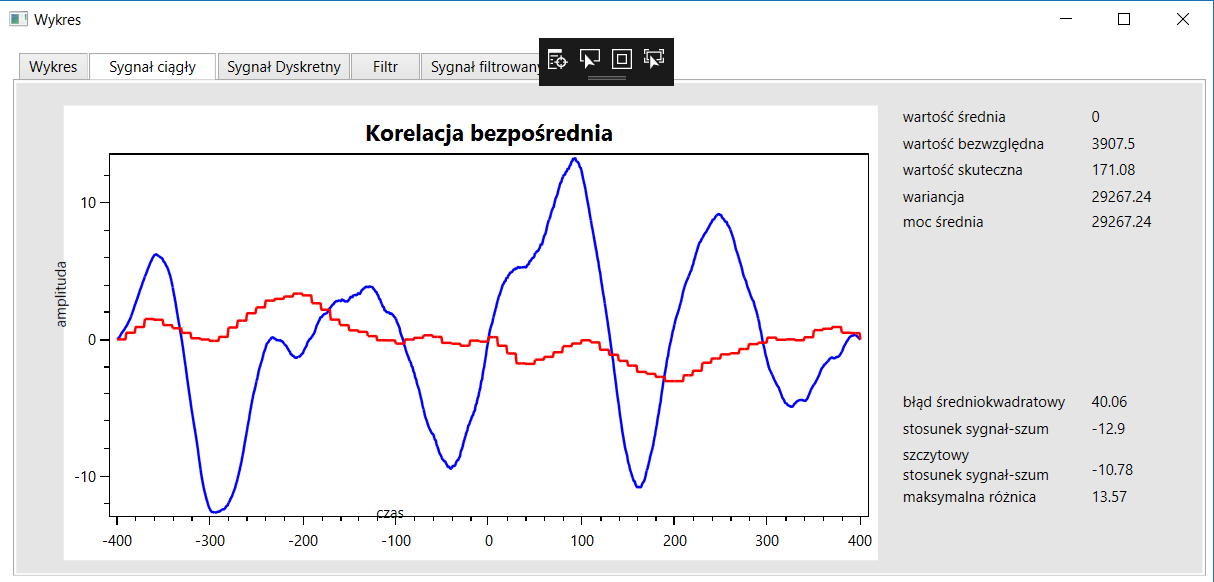
\includegraphics[width=12.3cm]{korBC.PNG}
 \vspace{-0.3cm}
 \caption{Wykres sygnału sinusoidalnego ciągły: kwantyzacja z obcięciem, interpolacja pierwszego rzędu}
 \label{Wykres dla wynikw eksperymentu pierwszego}
\end{figure}

\newpage
\begin{figure}[h!]
 \centering
 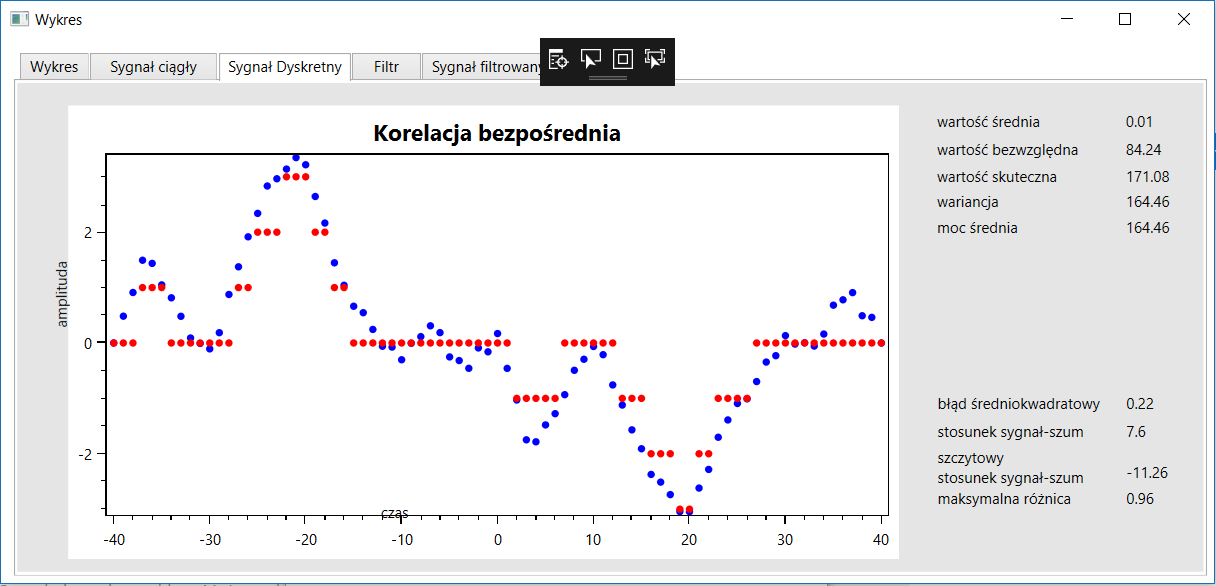
\includegraphics[width=12.3cm]{korBD.PNG}
 \vspace{-0.3cm}
 \caption{Wykres sygnału sinusoidalnego ciągły: kwantyzacja z obcięciem, interpolacja pierwszego rzędu}
 \label{Wykres dla wynikw eksperymentu pierwszego}
\end{figure}

Korelacja z wykorzystaniem splotu:
\\Rezultat przedstawia zamieszczony poniżej zrzut ekranu z programu. Wartości liczbowe oraz wykres funkcji amplitudy od czasu przedstawia \ref{Wykres dla wynikw eksperymentu pierwszego}.
\begin{figure}[h!]
 \centering
 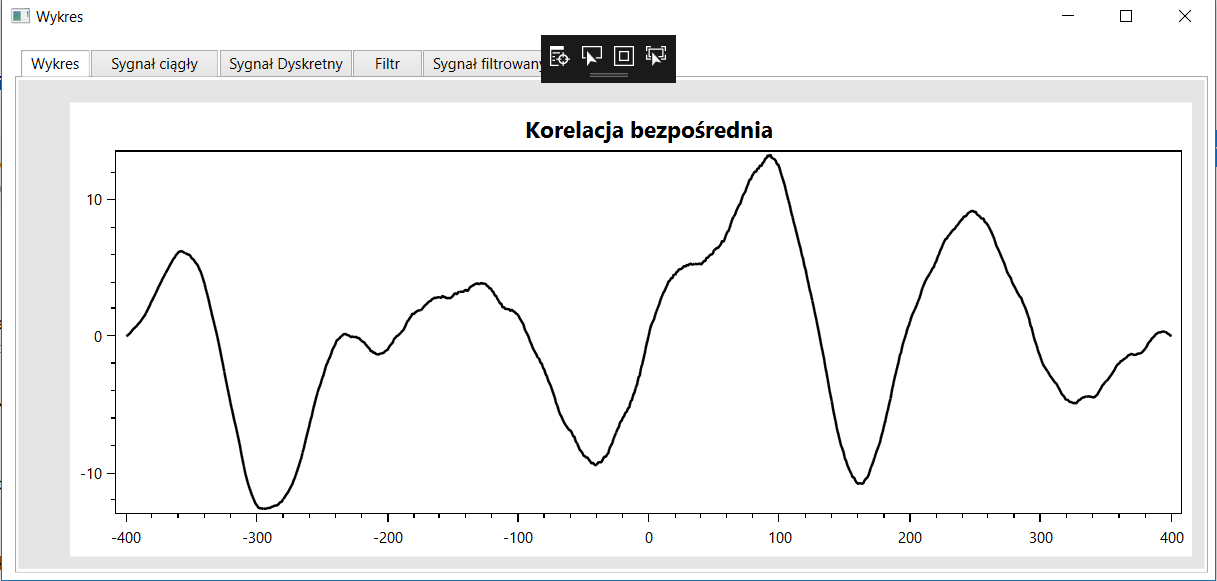
\includegraphics[width=12.3cm]{korB.PNG}
 \vspace{-0.3cm}
 \caption{Wykres sygnału sinusoidalnego ciągły: kwantyzacja z obcięciem, interpolacja pierwszego rzędu}
 \label{Wykres dla wynikw eksperymentu pierwszego}
\end{figure}
 \newpage
\begin{figure}[h!]
 \centering
 \includegraphics[width=12.3cm]{korBC.PNG}
 \vspace{-0.3cm}
 \caption{Wykres sygnału sinusoidalnego ciągły: kwantyzacja z obcięciem, interpolacja pierwszego rzędu}
 \label{Wykres dla wynikw eksperymentu pierwszego}
\end{figure}

\newpage
\begin{figure}[h!]
 \centering
 \includegraphics[width=12.3cm]{korBD.PNG}
 \vspace{-0.3cm}
 \caption{Wykres sygnału sinusoidalnego ciągły: kwantyzacja z obcięciem, interpolacja pierwszego rzędu}
 \label{Wykres dla wynikw eksperymentu pierwszego}
\end{figure}

%%%%%%%%%%%%%%%%%%%%%%%%%%%%%%%%%%%%%%%%%%%%%%%%%%%%%%%%%%%%%%%%%%%%%%%%%%%%%%%%%%%%%%%%%%%%%%%%%%%%%%%%%%%%%%%%%
% PODROZDZIA PT. EKSPERYMENT NR 6
%%%%%%%%%%%%%%%%%%%%%%%%%%%%%%%%%%%%%%%%%%%%%%%%%%%%%%%%%%%%%%%%%%%%%%%%%%%%%%%%%%%%%%%%%%%%%%%%%%%%%%%%%%%%%%%%%

\subsection{Eksperyment nr 6}

Eksperyment nr 6 - Radar\\

\subsubsection{Założenia}
Operacja splotu jest przeprowadzana dla dwóch dowolnych sygnałów dyskretnych o wczeniej podanych (niekonieczcnie jednakowych) ilosciach próbek. W tym celu jest wykorzystany wzór \ref{Splot_indeks}.

\subsubsection{Przebieg}
Do generacji synału prostokątnego zostały podane parametry:
\addtokomafont{labelinglabel}{\sffamily}

\begin{labeling}{szj}
\item [Amplituda (A):] 1
\item [Czas trwania (t1):] 100 s
\item [Częstotliwość próbkowania (d): ] 1 Hz
\item [Okres podstawowy :] 100 s
\item [Współczynnik wypełnienia:] 0,5
\end{labeling}

Wykres sygnału przedstawia poniższy obrazek:
\begin{figure}[h!]
 \centering
 \includegraphics[width=12.3cm]{prost.PNG}
 \vspace{-0.3cm}
 \label{gw}
\end{figure}
\subsubsection{Rezultat}

Opóźnienie = 5:
\\Rezultat przedstawia zamieszczony poniżej zrzut ekranu z programu. Wartości liczbowe oraz wykres funkcji amplitudy od czasu przedstawia \ref{Wykres dla wynikw eksperymentu pierwszego}.
\begin{figure}[h!]
 \centering
 \includegraphics[width=12.3cm]{prostR5.PNG}
 \vspace{-0.3cm}
 \caption{Wykres sygnału sinusoidalnego ciągły: kwantyzacja z obcięciem, interpolacja pierwszego rzędu}
 \label{Wykres dla wynikw eksperymentu pierwszego}
\end{figure}


Opóźnienie = 25:
\\Rezultat przedstawia zamieszczony poniżej zrzut ekranu z programu. Wartości liczbowe oraz wykres funkcji amplitudy od czasu przedstawia \ref{Wykres dla wynikw eksperymentu pierwszego}.
\begin{figure}[h!]
 \centering
 \includegraphics[width=12.3cm]{prostR25.PNG}
 \vspace{-0.3cm}
 \caption{Wykres sygnału sinusoidalnego ciągły: kwantyzacja z obcięciem, interpolacja pierwszego rzędu}
 \label{Wykres dla wynikw eksperymentu pierwszego}
\end{figure}

Opóźnienie = 50:
\\Rezultat przedstawia zamieszczony poniżej zrzut ekranu z programu. Wartości liczbowe oraz wykres funkcji amplitudy od czasu przedstawia \ref{Wykres dla wynikw eksperymentu pierwszego}.
\begin{figure}[h!]
 \centering
 \includegraphics[width=12.3cm]{prostR50.PNG}
 \vspace{-0.3cm}
 \caption{Wykres sygnału sinusoidalnego ciągły: kwantyzacja z obcięciem, interpolacja pierwszego rzędu}
 \label{Wykres dla wynikw eksperymentu pierwszego}
\end{figure}
\section{Wnioski}

Przeprowadzone eksperymenty dowodzą, że  Interpolacja pierwszego rzędu jest bardziej dokładna niż ekstrapolacja rzędu zerowego.  Dzieje się tak ponieważ między próbkami sygnał się zmienia zatem interpolowanie między kolejnymi próbkami daje lepsze odwzorowanie, niż przepisywanie tej samej wartości do czasu napotkania następnej próbki.
Aby uzyskać wyniki ekstrapolacji zbliżone do wyników ekstrapolacji należy przyjąć bardzo dużą częstotliwość próbkowania. Są znaczące róźnice w błędach odtworzenia sygnałów przez interpolację i ekstrapolację. Interpolacja jest dużo bardziej dokładna - błąd sredniokwadratowy o ok 0,2, stosunek sygnał-szum i szczytowy stosunek sygnał-szum różnią się nawet o 10 jednostek. Co ciekawe maksymalna różnica między sygnałem analogowym, a odtwarzanym sygnałem jest minimalnie większa dla interpolacji.
W przypadku kwantyzacji dużo lepiej sprawdza się kwantyzacja z zaokrągleniem. W przypadku kwantyzacji z obcięciem jeżeli próbkowaniem nie trafimy w szczyt amplitudy to maksymalna jej wartość po kwantowaniu będzie mniejsza niż ta w oryginale. Przy kwantyzacji z zaokrągleniem unikamy takiej sytuacji.
Podczas próbkowania trzeba bardzo uważać przy podawaniu częstotliwości. Jeśli podamy ją zbyt mała sygnał nie zostanie odtworzony, a czasem wręcz możemy uzyskać inny sygnał.
%%%%%%%%%%%%%%%%%%%%%%%%%%%%%%%%%%%%%%%%%%%%%%%%%%%%%%%%%%%%%%%%%%%%%%%%%%%
% PODROZDZIA PT. ZALACZNIKI
%%%%%%%%%%%%%%%%%%%%%%%%%%%%%%%%%%%%%%%%%%%%%%%%%%%%%%%%%%%%%%%%%%%%%%%%%%%
\begin{thebibliography}{0}
   \bibitem{l2short} FTIMS Politechnika Łódzka.
    \textsl{Przetwarzanie sygnałów, pojęcia podstawowe Plik}, Wikamp.
 \bibitem{l2short} FTIMS Politechnika Łódzka.
    \textsl{Zadanie 2 Generacja sygnału i szumu}, Wikamp.
\end{thebibliography}

\end{document}